%% ----------------------------------------------------------------
%% Thesis.tex -- MAIN FILE (the one that you compile with LaTeX)
%% ---------------------------------------------------------------- 

% Set up the document
\documentclass[a4paper, 12pt, oneside]{Thesis}  % Use the "Thesis" style, based on the ECS Thesis style by Steve Gunn
\usepackage{graphicx}
\graphicspath{Figures/}  % Location of the graphics files (set up for graphics to be in PDF format)

% Include any extra LaTeX packages required
\usepackage{tikz}
\usepackage{natbib}  % Use the "Natbib" style for the references in the Bibliography
\bibliographystyle{agsm}
\renewcommand{\bibname}{References}
\usepackage{verbatim}  % Needed for the "comment" environment to make LaTeX comments
\usepackage{vector}  % Allows "\bvec{}" and "\buvec{}" for "blackboard" style bold vectors in maths
\hypersetup{urlcolor=blue, colorlinks=true}  % Colours hyperlinks in blue, but this can be distracting if there are many links.

%% ----------------------------------------------------------------
\begin{document}
\frontmatter     % Begin Roman style (i, ii, iii, iv...) page numbering
% Set up the Title Page
\title  {A systematic exploration of food recognition using computer vision techniques}
\authors  {Laurynas Tumosa}
            
\addresses  {\groupname\\\deptname\\\univname}  % Do not change this here, instead these must be set in the "Thesis.cls" file, please look through it instead
\date       {\today}
\subject    {}
\keywords   {}

\maketitle
%% ----------------------------------------------------------------

\setstretch{1.3}  % It is better to have smaller font and larger line spacing than the other way round

% Define the page headers using the FancyHdr package and set up for one-sided printing
\fancyhead{}  % Clears all page headers and footers
\rhead{\thepage}  % Sets the right side header to show the page number
\lhead{}  % Clears the left side page header

\pagestyle{fancy}  % Finally, use the "fancy" page style to implement the FancyHdr headers

%% ----------------------------------------------------------------
% Declaration Page required for the Thesis, your institution may give you a different text to place here
%\iffalse
\Declaration{

\addtocontents{toc}{\vspace{1em}}  % Add a gap in the Contents, for aesthetics

I certify that the material contained in this dissertation is my own work and does not contain unreferenced or unacknowledged material. I also warrant that the above statement applies to the implementation of the project and all associated documentation. Regarding the electronically submitted version of this submitted work, I consent to this being stored electronically and copied for assessment purposes, including the School's use of plagiarism detection systems in order to check the integrity of assessed work.
I agree to my dissertation being placed in the public domain, with my name explicitly included as the author of the work. \\

Date:\\  % This prints a line to write the date
\rule[1em]{25em}{0.5pt}

Signed:\\
\rule[1em]{25em}{0.5pt}  % This prints a line for the signature
\\
\addtotoc{Working Documents}  % Add the "Abstract" page entry to the Contents
\work{
\addtocontents{toc}{\vspace{1em}}  % Add a gap in the Contents, for aesthetics

The working documents of this project are availabe at \url{https://github.com/laur1s/FoodClassifier} and \url{http://www.lancaster.ac.uk/ug/tumosa/}. A food image dataset used is made available at \url{https://lancaster.app.box.com/v/FoodData}.
The \LaTeX\     source code of this  report is available at \url{https://github.com/laur1s/Dissertation}.
}
 
 
}
\clearpage  % Declaration ended, now start a new page

%% ----------------------------------------------------------------
% The "Funny Quote Page"
%\pagestyle{empty}  % No headers or footers for the following pages

%\null\vfill
%% Now comes the "Funny Quote", written in italics
%\textit{``Write a funny quote here.''}

%\begin{flushright}
%If the quote is taken from someone, their name goes here
%\end{flushright}

%\vfill\vfill\vfill\vfill\vfill\vfill\null
%\clearpage  % Funny Quote page ended, start a new page
%% ----------------------------------------------------------------

% The Abstract Page
\addtotoc{Abstract}  % Add the "Abstract" page entry to the Contents
\abstract{
\addtocontents{toc}{\vspace{1em}}  % Add a gap in the Contents, for aesthetics

The dissertation focuses on computer vision techniques for classifying food objects from images. Food classification is an important task, that could be use for automatic dietary assessment.To accomplish this task, the dataset of food images was firstly obtained. Then, different machine learning algorithms such as the  k-nearest neighbors classifier, support vector machine, linear classifier, multilayer neural network, convolutional neural network, and transfer learning were explored. The classifiers that use these algorithms were developed. To evaluate the classification performance, accuracy score of each classifier was calculated. The method that worked best, transfer learning, achieved 98.20 percent accuracy on the test dataset. It was concluded that food classification from images with reasonable accuracy was possible and deep learning models work much better for this task, compared to the other machine learning techniques.

}

\clearpage  % Abstract ended, start a new page
     

%% ----------------------------------------------------------------

\setstretch{1.3}  % Reset the line-spacing to 1.3 for body text (if it has changed)
% The Acknowledgements page, for thanking everyone
\acknowledgements{
\addtocontents{toc}{\vspace{1em}}  % Add a gap in the Contents, for aesthetics

I would like to thank to my project supervisor, Adrian Friday for guidance and valuable feedback provided for implementing  the project and writing the report.

I would like to thank Christian Bizer who taught a data mining course at the University of Mannheim when I studied there. This course introduced me to data mining and machine learning  and aroused my interest in this field of computer science.

I would like to thank Andrej Karpathy who was a lecturer at Stanford's CS231n: Convolutional Neural Networks for Visual Recognition course. He made all  lecture recordings and the course material publicly available. These lectures were a great learning material and contrbuted greatly to the success of the project.

I would like to thank my family for believing that I could study computer science at university and for supporting and encouraging me.

Finally, I would like to dedicate this dissertation to my sister, Aiste.

}
\clearpage  % End of the Acknowledgements

\pagestyle{empty}  % Page style needs to be empty for this page
%\addtotoc{Dedication}
%\addtocontents{toc}{\vspace{1em}} 
%\dedicatory{Dedicated to my sister Aiste}

%% ----------------------------------------------------------------

\pagestyle{fancy}  %The page style headers have been "empty" all this time, now use the "fancy" headers as defined before to bring them back


%% ----------------------------------------------------------------
\lhead{\emph{Contents}}  % Set the left side page header to "Contents"
\tableofcontents  % Write out the Table of Contents

%% ----------------------------------------------------------------
\lhead{\emph{List of Figures}}  % Set the left side page header to "List if Figures"
\listoffigures  % Write out the List of Figures

%% ----------------------------------------------------------------
\lhead{\emph{List of Tables}}  % Set the left side page header to "List of Tables"
\listoftables  % Write out the List of Tables

%% ----------------------------------------------------------------
\setstretch{1.5}  % Set the line spacing to 1.5, this makes the following tables easier to read
\clearpage  % Start a new page
\lhead{\emph{Glossary}}  % Set the left side page header to "Abbreviations"
\listofsymbols{ll}  % Include a list of Abbreviations (a table of two columns)
{
% \textbf{Acronym} & \textbf{W}hat (it) \textbf{S}tands \textbf{F}or \\
\textbf{ReLU} & rectified linear unit\\
\textbf{K-NN algorithm} & k-nearest neighbors algorithm\\
\textbf{SVM} & support vector machine\\
\textbf{CNN} & convolutional neural network\\


}


%% ----------------------------------------------------------------
% End of the pre-able, contents and lists of things
% Begin the Dedication page

\setstretch{1.3}  % Return the line spacing back to 1.3



%\addtocontents{toc}{\vspace{2em}}  % Add a gap in the Contents, for aesthetics

%% ----------------------------------------------------------------
\mainmatter	  % Begin normal, numeric (1,2,3...) page numbering
\pagestyle{fancy}  % Return the page headers back to the "fancy" style

% Include the chapters of the thesis, as separate files
% Just uncomment the lines as you write the chapters
%\fi

\chapter{Introduction}
\lhead{\emph{Introduction}}

Food is a very important part of everyone’s life.  One of the common sayings about food is ``You are what you eat" meaning that eating healthy food like vegetables and fruits will make one healthier and eating fast food is bad for one’s body.  

Tracking what one eats is really helpful for maintaining a healthy diet or losing weight. Since these days we are living in such a fast-paced world it is often hard to keep track of food that one eats during the day. Weight and calorie intake apps for smartphones are getting more popular since they allow users to capture their food intake on the go. However, an approach that today’s mobile applications use for entering food intake is obtrusive and not very user-friendly. Users are required to open their food diary applications and search for the eaten food using their smartphones' keyboards. 

The goal of this project is to explore techniques for an automatic food classification form images. This could enable users to capture food that they eat in an unobtrusive and user-friendly way. A created machine learning model could use a picture of a food taken by a smartphone's camera as an input method and classify it. In most of the smartphones, a camera can be accessed in a few clicks. People are used to taking pictures on their smartphones. Therefore, an automatic food classification using phone camera would be a perfect solution to the food tracking problem. 

However, automatic food classification in not an easy task. There is no direct way to detect what kind of food product is in a picture. the digital image is just a matrix of numbers representing an intensity of three different color components: red, green and blue (RGB) it is impossible to create an algorithm that could directly map image to the label of a food item. Therefore, a machine learning is needed to learn a model that can recognize a specific type of food from an image and differentiate between various types of food. Machine learning is the subfield of computer science that gives computers the ability to learn without being explicitly programmed \citep{Samuel}.

Supervised learning is a machine learning task for mapping labeled examples as training data and makes label predictions for all unseen points \citep{Mohri:2012:FML:2371238}. This project explores various supervised learning algorithms that could be used for classifying the images as well as techniques for image processing for machine learning.

The aims of the project are to explore the machine learning algorithms that could be used for food image classification.
Then, these algorithms are going to be systematically evaluated and their performance is going to be compared.

The key challenges, that are going to be faced are the generation of a food image dataset, preprocessing of images and creating and training of machine learning algorithms.

\section{The structure of the report}
In the next chapter, background theory and research work in this area are going to be introduced. Chapter 3 presents the chosen programming language and machine learning library, as well as evaluation method used to track the performance of the algorithms used. Chapter 4 displays why a dataset of food images was needed, what kind of requirements were set for it and how was it downloaded. In Chapter 5 implementation details of machine learning algorithms are described. Each algorithm is firstly shortly introduced, then implementation details are provided and finally, it's classification results are shown.  In Chapter 5 a specific type of machine learning- deep learning is explored. Chapter 6 compares the best results of all classifiers that were built. Finally, in chapter 7 the conclusions are derived. % Introduction

\chapter{Background}
\lhead{\emph{Background}}

\section{Introduction to the history of computer vision}
\label{sec:intro}


Computer vision is a relatively old field in computer science. The subject itself has been around since the 1960s, but it is only recently that it has been possible to build useful computer systems ideas from computer vision \cite {cv}.
The birthday of Computer Vision is considered the summer of 1966.  During that year a computer vision summer project was proposed in MIT AI lab \citep{papert}. The goal of the summer vision project was to use summer workers (students) effectively in the construction of a significant part of a visual system. It was thought that a vision was a relatively easy field of AI and that a landmark in the development of pattern recognition could be created during the summer. The task, however, was a lot harder than previously expected and no significant computer vision problems were solved during that project.

During development of a computer vision, it was noticed that is very hard to recognize an object by describing the whole image because of the pixel variation in images that are produced under different conditions. Important features have to be selected to make an image more resistible to various variations. Later these selected features are used for detecting a specific object. In 1999 a new method for image feature generation called the Scale Invariant Feature Transform (SIFT) was proposed by \cite{sift}. These features are invariant to image scaling, translation, and rotation, and partially invariant to illumination changes. Because of that SIFT features performed much better than correlation-based template matching technique that was used before and could be seen as a major break point in computer vision.
 
Another method for detecting features in images was proposed by \citep{nakano2006object}. This paper states that since objects are composed of a combination of characteristic parts, a good object detector could be developed if local parts specialised for a detection target are derived automatically from training samples. To do this, Independent component analysis (ICA) was used which decomposes a signal into independent elementary signals. Then ICA vectors were applied to the candidate area and their outputs were used in classification. Using this approach face detector algorithm used in Fujifilm camera with real-time face detection was created. It is considered to be a first commercial application that could run computer vision algorithms in real time. 
 
The important turning point in the development of computer vision field was a creation of ImageNet dataset and the ImageNet Large Scale Visual Recognition Challenge in 2010. The challenge is a competition where research teams submit image classification algorithms that classify and detect objects and scenes. The challenge is running annually since 2010 \citep{ImageNet}. In 2010 the goal of the challenge was to estimate the content of photographs for the purpose of retrieval and automatic annotation using a subset of the large hand-labeled ImageNet dataset (10.000.000 labeled images depicting 10.000+ object categories) as the training set. Example images which represent a pizza class can be seen in \autoref{fig:imgnet}.


Because of a  big amount of images and categories ImageNet was and still is a huge challenge for researchers who compete in the challenge.  ImageNet encouraged improvement and innovation in computer vision techniques. In 2012 ImageNet competition was won by an approach that used convolutional neural networks- AlexNet \citep{alex}. Since then deep learning became a dominant method for an image classification. 


 \begin{figure}[h]
\centering
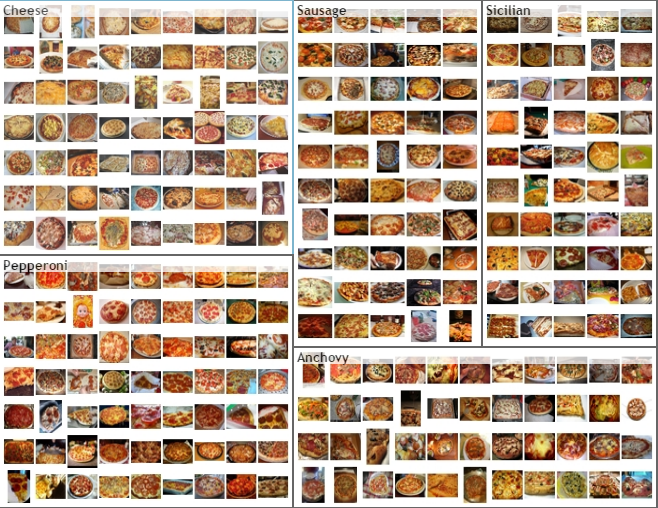
\includegraphics[width=10cm]{Figures/2/imgnet.PNG}
\caption{Example images with a pizza class label from the ImageNet }
\label{fig:imgnet}
\end{figure}


\section{Why is computer vision a hard problem?}
The true challenge to artificial intelligence proved to be solving the tasks that are easy for people to perform but hard for people to describe formally – problems that we solve intuitively, that feel automatic, like recognizing objects in images \citep{Goodfellow-et-al-2017}.

A human can recognize objects in images under all kinds of variations of illumination, viewpoint, scale, etc. In comparison, computer algorithms are very susceptible to all kinds of variations in images. Major variations in images were defined by \cite{231n} as:

\begin{enumerate}
\item Viewpoint variation. A single instance of an object can be oriented in many ways with respect to the camera.
\item Scale variation. Visual classes often exhibit variation in their size (size in the real world, not only in terms of their extent in the image).
\item Deformation. Many objects of interest are not rigid bodies and can be deformed in extreme ways.
\item Occlusion. The objects of interest can be occluded. Sometimes only a small portion of an object can be visible.
\item Illumination conditions. The effects of illumination are drastic on the pixel level.
\item Background clutter. The objects of interest may blend into their environment, making them hard to identify.
\item Intra-class variation. The classes of interest can often be relatively broad, such as a chair. There are many different types of these objects, each with their own appearance.
\end{enumerate}


 \begin{figure}[h]
\centering
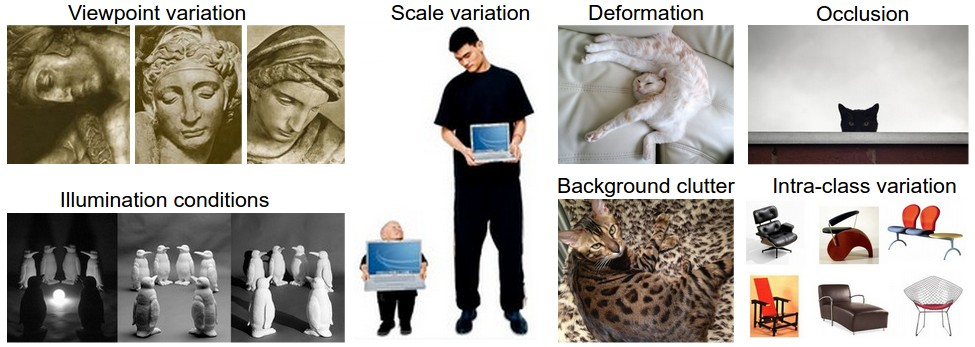
\includegraphics[width=14cm]{Figures/2/challenges.jpeg}
\caption{Example of various variations in images \citep{231n}}
\label{fig:imgnet}
\end{figure}

The actual solution of the variation problem still has not been found. Currently, this problem is either ignored or some algorithms that are partly resistant to variations are used.

\section{Saliency-aware food image segmentation for personal dietary assessment using a wearable computer}
A computer system that can be used for an image-based dietary assessment was described by \cite{chen2015saliency}. A wearable computer called eButton is used to capture the eating events. The eButton is a small, unobtrusive chest fob that can be pinned to clothing on the chest. Its camera takes pictures automatically at a rate of one picture per second during eating events. Then segmentation techniques are applied to segment a food from a container. Finally, a person manually enters the food label to the application. Later food volume is estimated. There is no information about food volume measurement, nutrient database lookup and calculation of calories in the paper despite that these steps are shown in the eButton operational diagram. \autoref{fig:1}
\begin{figure}[ht]
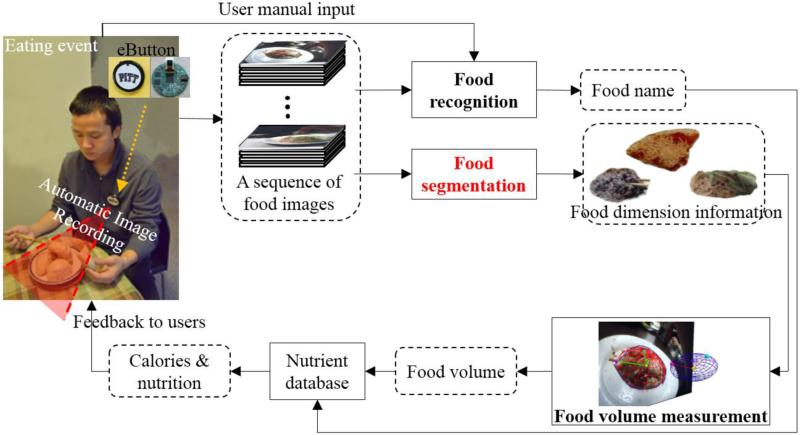
\includegraphics{Figures/segm_01.jpg}
\caption{Personal dietary assessment using a wearable computer eButton. }
\label{fig:1}
\end{figure}

The main focus of the paper is food segmentation from its container. It states that major difficulties in automatic food segmentation are multiple food components in complex and varying configurations, colored decorative patterns on plates and occlusion by non-food objects. The example images of these three difficulties are shown in  \autoref{fig:2}.

\begin{figure}[ht]
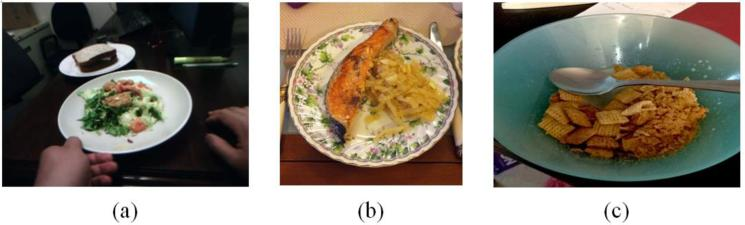
\includegraphics{Figures/segm_02.jpg}
\caption{Major difficulties in automatic food segmentation }
\label{fig:2}
\end{figure}

Researchers use two stages approach for food segmentation. Firstly, food container is detected in an image. The container is detected by shape convexity.  Canny edge detector is used to obtain the edge information from a given image.
Then, a number of square windows centered at edge pixels are randomly selected \label{fig:2}. A trained support vector machine with the histogram of a gradient as the classifier input is used to discard the non-container edge windows, increasing the detection efficiency. 

For detecting the food inside a plate researchers used color contrast to characterize the difference between the objects in the region against their surroundings, color abundance to characterise a probability of a color appearing in the local window and spatial arrangement to recognize the areas with one highly dominant color in the image. These 3 characteristics are then combined into one function.

The data set used to evaluate the segmentation approach in this research was combined from 30 eating events captured with eButton and 30 food images from the Jawbone database. Accuracy was measured by visually inspecting the quality of the segmentation and by comparing the image segmented by a computer to the images segmented by two research participants and measuring the difference. 



\begin{figure}[ht]
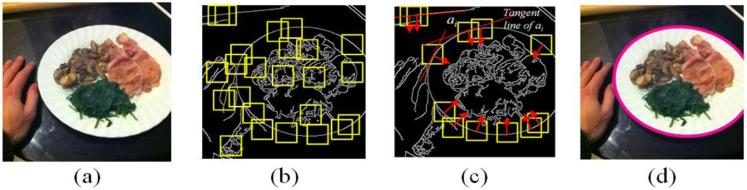
\includegraphics{Figures/2/segm_03.jpg}
\caption{Container detection}
\label{fig:3}
\end{figure}

The main limitation of this approach is that in some cases food is served not in a round shaped container e.g.: take away food box, lunch box which is usually rectangular. Some of the foods can also be eaten without using any container at all e.g: fruits, vegetables.

\iffalse
\section{Food-101 Mining Discriminative components with random forests}
This paper address the problem of automatically recognizing pictured dishes. A novel method is proposed to mine discriminative parts using Random Forests, which allowed to mine for parts simultaneously for all classes and to share knowledge among them.
A dataset of 101 food categories, with 101’000 images, was created by the authors of the paper.  Random forest classification method produced an average accuracy of 50.76 percent.
\fi
\section{Survey of calorie counter applications}

To get a better understanding what are the input methods offered by currently available calorie counter it was decided to try them. To download the apps keyword \"calorie counting\" was entered into the search bar of Google Play Store. The top 3 apps in the search results were downloaded and tested. These apps were MyFitnessPal, Nutracheck, and Lifesum.

MyfitnessPal is the most popular calories Counting app on the Google Play Store. The app has over 50 million downloads on Google Play Store \autoref{fig:mfp}. When the app is launched for the first time the user is required to sign up. After entering his email and password the user has to complete a short survey about his goal, physical activity levels, gender, birthday, location, weight, and height, desired weight and agree to the privacy policy and terms \autoref{fig:mfp2}. After that, the app calculates target daily calorie intake. For entering food user can scan the barcode of the food or use the text-based search. Food search and barcode scanning only work when a phone is connected to the Internet.  The database of food items is quite big and includes products from many different restaurants. However,  adding a meal that was prepared by the user himself is complicated. Every ingredient of a dish must be searched and added separately.  The portion size has to be entered using weight measurements e.g.:  grams. It is often hard to estimate how much does a meal weight so it is a big disadvantage.
 
\begin{figure}[ht]
\centering
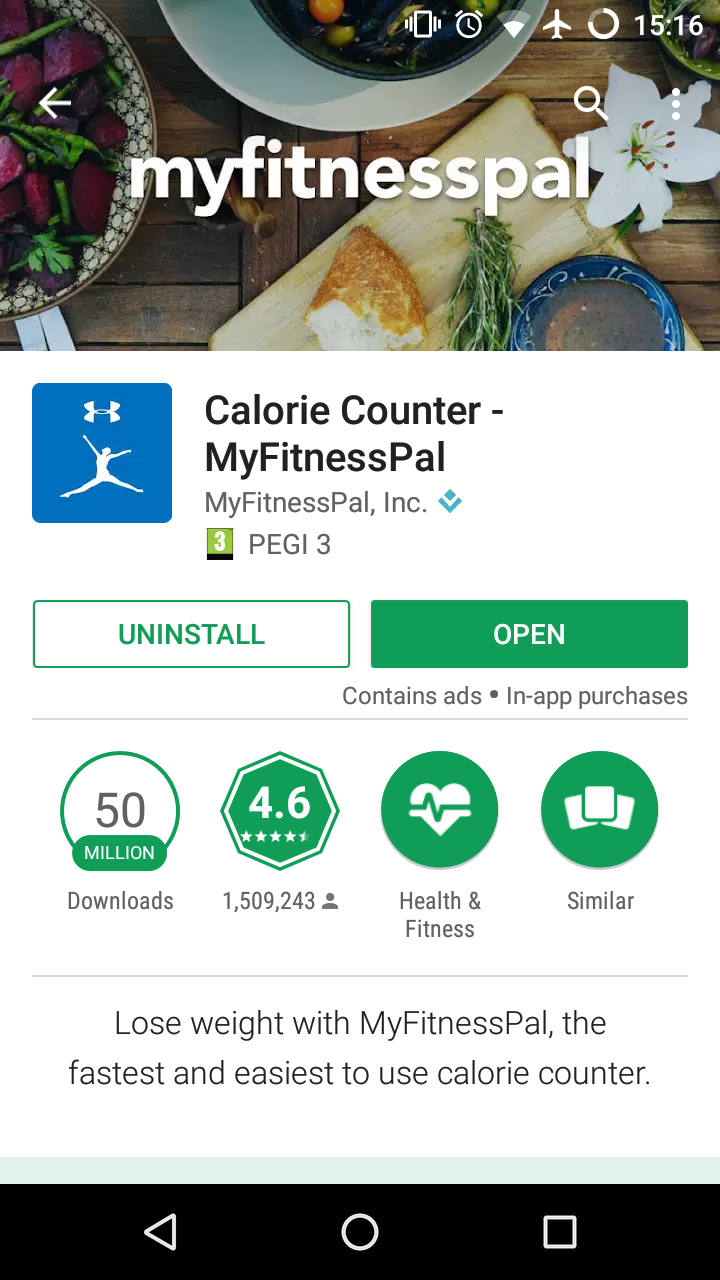
\includegraphics[width=5cm,scale=0.5]{Figures/2/mfp1.png}
\caption{Google Play Store page of MyFitnessPal app}
\label{fig:mfp}
\end{figure}

\begin{figure}[ht]
\centering
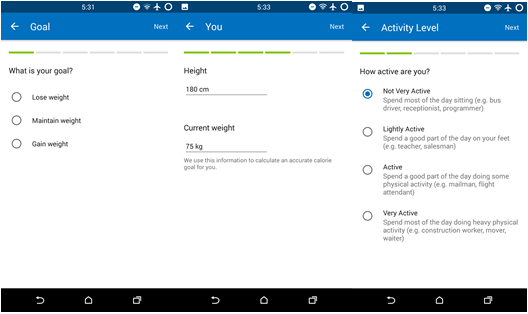
\includegraphics[width=10cm]{Figures/2/mfp2.png}
\caption{Procedure to create a MyFitnessPal account}
\label{fig:mfp2}
\end{figure}

\begin{figure}[ht]
\centering
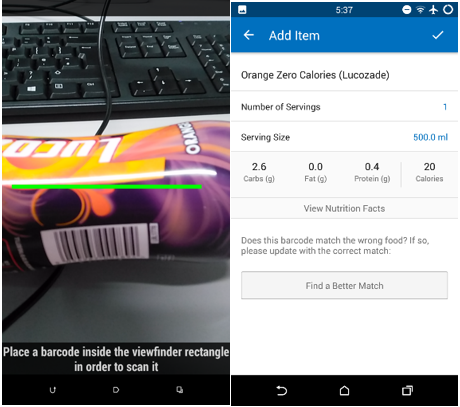
\includegraphics{Figures/2/mfp3.PNG}
\caption{Barcode scanning with MyFitnessPal}
\label{fig:mfp2}
\end{figure}

The other app tested was Nutracheck. To start using Nutracheck a user is required to create an account. The registration procedure is very similar to MyFitnessPal's. For entering meals, the app also has a barcode scanner and search function.  The advantage that Nutracheck has over MyFitnessPal is that it displays images of food in the search results \autoref{fig:eat}. However, a  barcode scanner of this app recognized fewer barcodes that a barcode scanner in MyFitnessPal.

Final app that was tested was Lifesum. It also requires completing a survey in order to start using it and uses a barcode scanner and a search function for adding food. An interesting feature that this app has compared to other apps is food quality rating. It rates a quality of a food according to it nutrition facts and presents the user with a rank of food from A to F \autoref{fig:life}.

 \begin{figure}[ht]
\centering
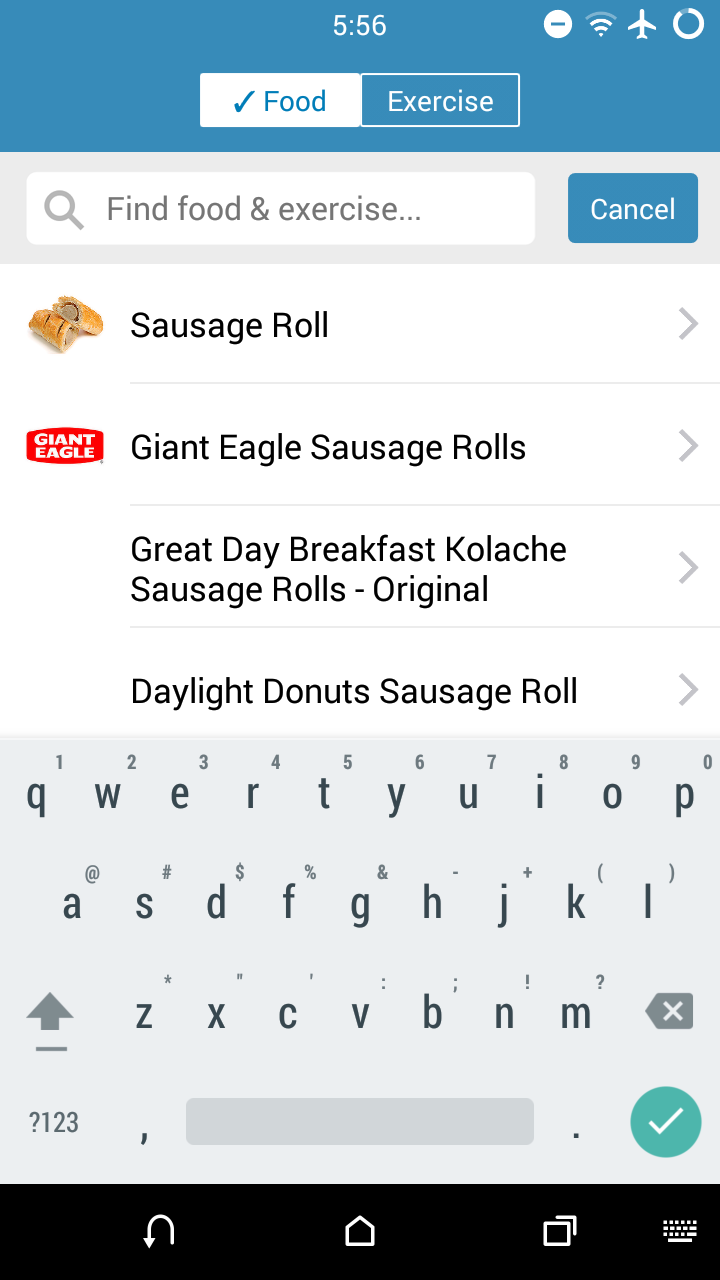
\includegraphics[width=5cm]{Figures/2/eat.png}
\caption{Food database search in Nutracheck}
\label{fig:eat}
\end{figure}

\begin{figure}[ht]
\centering
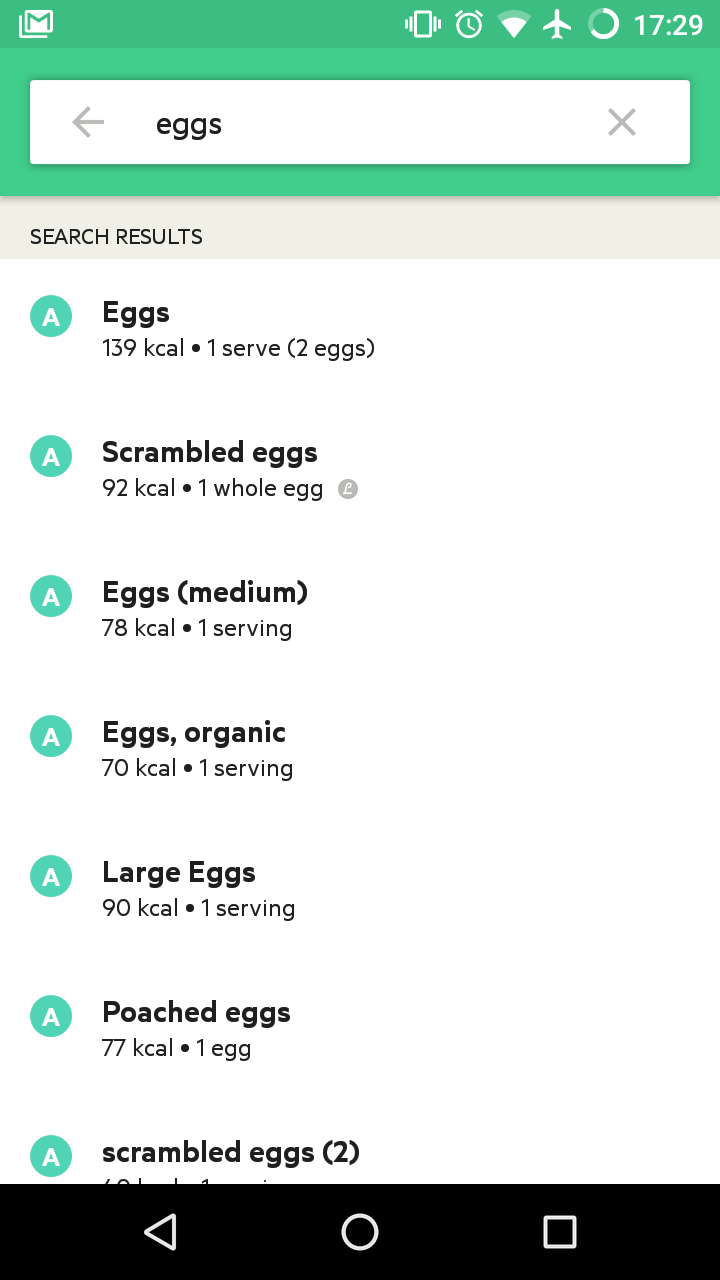
\includegraphics[width=5cm]{Figures/2/mm.png}
\caption{Food database search in LifeSum}
\label{fig:life}
\end{figure}

From this short survey, it can be concluded that currently, available calorie counting apps lack innovation. They all use text-based search and barcode scanners as data entry points. If one wants to track his food, he must remember what did he eat and estimate how much did It weight. All tried apps require an Internet connection for entering food for tracking.  It is clear, that food tracking applications could benefit from a model that can recognize and classify food from images.

\section{Summary}
In this chapter history of computer vision was reviewed. Then, it was explained why computer vision is such a hard problem. Finally, a  paper about automatic food image segmentation was summarized and reviewed. This paper explored dietary assessment only focusing on segmenting a food object from a background. An automatic food image classifier could extend the capabilities of personal dietary assessment with wearable devices. In the next chapter research methods of the project is going to be discussed. % Background Theory 

\chapter{Research Methods}
\lhead{\emph{Research Methods}}

This chapter provides information about the research methods used in this project. Before conducting a series of experiments, to explore and evaluate machine learning methods, it was needed to decide on how are these algorithms going to be implemented and evaluated. Choices of a programming language,  a machine learning library, and an evaluation method are explained in this chapter.

\section{Choice of a Programming Language}

 It was chosen to use Python programming language for implementing this project. The language was chosen because it is one of the most popular languages used by machine learning researchers and developers. It is also free and open source. Since Python is an interpreted language, code written in Python can be executed on multiple different platforms without having a need to modify the code. Because  Python language has a large community of developers, there are many publicly available open source packages with efficient implementation of machine learning algorithms for this language.

Availability of scientific computing tools for Python was also one of the main reasons why this language was chosen. Scientific Python libraries that were used in this project were Matplotlib, NumPy, IPython and Jupyter Notebook \citep{scipy}. Matplotlib provided an ability to plot graphs, images, and tables. NumPy was used for efficient arithmetical operations with matrices. IPython allowed executing only a part of a program without a need to run a full code. It is a system for an interactive scientific computing \citep{ipython}. Some of the operations, for example, loading the dataset or resizing the images can take a long time to complete. In IPython these operations are only required to be completed once. Then, results of these operations are saved in memory where they remain and can be reused. Jupyter Notebook allowed to execute Python code in a web browser and save the results as HTML pages (\autoref{fig:jupyter}). Jupyter Notebook is an IPython wrapper that launches an HTTP server. Scientific Python libraries allowed to interactively explore the data with an ability to plot graphs, tables and visualise results.

The alternative language that was also considered was Matlab. Matlab is a domain specific programming language that was designed specifically for matrix programming. It also includes an image processing and machine learning toolboxes. Machine learning and image processing functions are easier to use in Matlab than in Python because this language was developed for a particular purpose. However, Matlab is a closed source language. It also only supports some platforms, where Python code can be executed in almost any computing environment. Therefore, Python programming language was a better option.

\begin{figure}[ht]
\centering
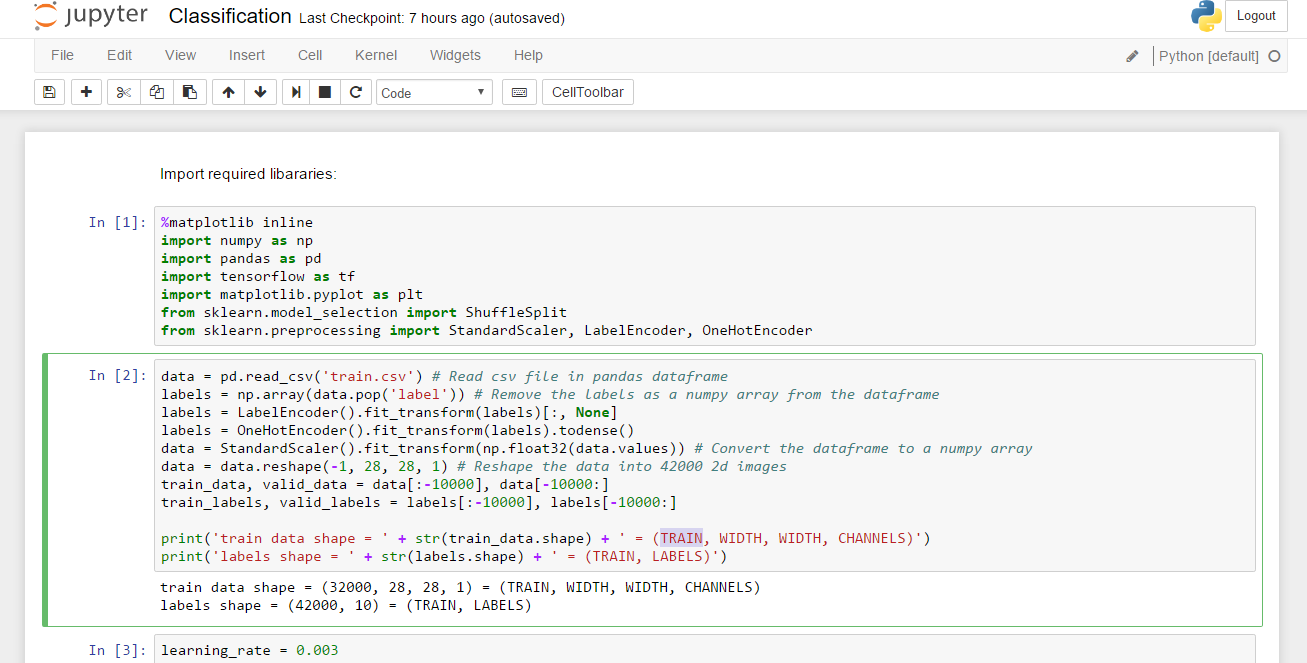
\includegraphics[width=14cm]{Figures/c3/c3jupyter.PNG}
\caption{Example of a Jupyter Notebook}
\label{fig:jupyter}
\end{figure}


\section{Choice of Machine learning libraries}

\subsection{Why was a Machine Learning Library Needed?}

It is possible to implement machine learning algorithms without using any additional library. However, there are many benefits provided by machine learning libraries. Algorithms available in machine learning libraries are often implemented more efficiently. Adapting a provided algorithm for a specific task also takes a less time than  writing a particular algorithm for it. Therefore, it was decided to analyse what machine learning libraries are available for Python.

\subsection{Library Used for Machine Learning }

Sckit-learn python package was chosen as a library for working with machine learning models. This package provides state-of-the-art implementations of many well-known machine learning algorithms and has an easy-to-use interface tightly integrated with the Python language \citep{pedregosa2011scikit}. Large parts of this module are written in C or C++. Because C and C++ are much faster than Python, it makes algorithms run faster compared to a standard Python implementation. Sckit\-learn machine learning algorithms are high-level API's \citep{buitinck2013api}. Algorithms provided in this package do not require a knowledge of their implementation details. Nevertheless, Sckit-learn interface allows parameters of these algorithms to be configured.

In the case of food image classification, the main advantages that Sckit-learn provided were the fact that it uses the same data input format for every machine learning algorithm and ability to easily configure parameters, to make classifiers work on image classification.


\section{The Evaluation Method for the Classification Algorithms}

The key indicator of performance in the classification task is a classification accuracy. Accuracy is calculated by dividing the number of correct predictions by the total number of predictions. By calculating and comparing accuracy scores for every machine learning algorithm tried, the best food image classification technique was found.

Other helpful performance indicators used to evaluate a classification performance when parameters of classification algorithms were tuned were: confusion matrix, precision, recall and f measure. Confusion matrix shows how often and what classes are misclassified as other classes. Precision is the total number of elements classified correctly divided by a total number of items that were classified as that class. A recall is the total number of objects classified correctly divided by a total number of items of that type in the database. A graphical illustration of precision and recall measures is shown in \autoref{fig:p}.  F-measure is a measure combined from precision and recall according to a formula \( F = 2 \frac{Recall \times Precision }{Recall  +  Precision} \)   \citep{ting2011}. 


\begin{figure}[ht]
\centering
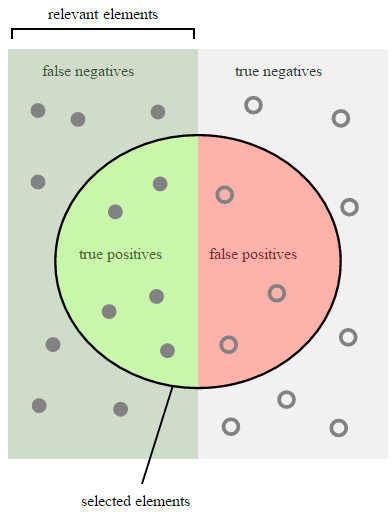
\includegraphics[width=5cm]{Figures/Capture.PNG}
\caption{Precision and Recall \citep{wiki:p}}
\medskip
\( P =\frac{TP}{TP+ FP}\),
\( R =\frac{TP}{TP+ FN}\)
\label{fig:p}
\end{figure}


\section{Summary}
In this chapter reasoning behind a chosen programming language and machine learning library used was provided. Methods for evaluating the performance of classification algorithms were discussed. Accuracy score was picked as the primary method for performance evaluation. In the following chapter, accumulation of a food image dataset is discussed. % Methods

\chapter{Accumulation of a Food Image Dataset}
\lhead{\emph{Accumulation of a Food Image Dataset}}

Before starting to experiment with machine learning algorithms for food classification, a dataset of food images needed to be created. In this chapter, reasons, why the dataset is required, are going to be explained and a process of accumulating the dataset is going to be described.

\section{The Requirements for the Food Image Dataset}
 The dataset was needed because classification algorithms use the dataset to learn a classification model from it. The most important requirements to the dataset were:

\begin{enumerate}
  \item The images of the dataset should be taken under a real life conditions.
  \item There should be enough pictures in the dataset to learn the model for every machine learning algorithm that is going to be tried.
  \item Variance of food images of the same class should be high. 
\end{enumerate}

Real life condition pictures were needed, because of the intention to create a model that could classify pictures of food taken by people using cameras of mobile phones, it was critical that food images in the dataset could not be created in lab conditions. People use different angles and distance for taking pictures. The light conditions in images often vary greatly too. It was crucial to represent these conditions in the food image dataset.

The dataset also needed to have many images belonging to each class. Having a lot of training samples is the best way to make sure that the model learned is generalised enough to perform well on a test dataset. Simple models trained on a lot of data perform better than more elaborate models based on less data \citep{unreasonable}.Because of that, it was decided that around 1,000 training images are needed for each class of food in the dataset. 

Finally, an intraclass class variance of pictures in the training dataset should also be high. The problem of datasets with little variance can be illustrated with a dataset of tree images containing only pictures of trees with green leaves.The model learned by a classifier from this dataset will always classify a tree with orange leaves or a tree without leaves as a not tree. Therefore, a food dataset should also include a different kind of images for the same class e.g. pizza with cheese, pepperoni pizza, a slice of pizza, etc. 

Accumulation of the dataset that satisfies these requirements was a challenging task. It would take a long time to take enough photos of meals for creating a big enough dataset. Also, a dataset containing images taken by only one or a few persons would not have enough variance. Because of that, possibilities to download food images from the Internet had to be explored.


It was observed that there are a lot of food images hosted on a photo sharing service flickr.com. After reading that Flickr has a Python API that could be used for searching for images according to their tags or titles and then downloading these images resized to the specified resolution, it was decided to write a Python script using this API. After downloading the images with a tag ``Fish and Chips",  it was realized that there were a lot of images that contained this tag but were not actual food pictures e.g. \autoref{fig:fish}. Because of the time it takes to review every image downloaded and delete pictures that do not represent the class, it was decided to try to find a public food image dataset with images that were already classified.  


\begin{figure}[ht]
\centering
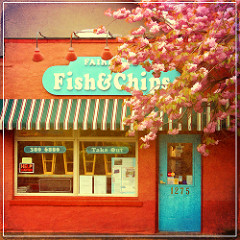
\includegraphics[width=2cm]{Figures/c3/flick.jpg}
\caption{Example of an image with a fish and chips tag, downloaded using the Flickr API}
\label{fig:fish}
\end{figure}


It was found that ImageNet Classification challenge, that was briefly described in \autoref{sec:intro}  includes many categories of food pictures. The only problem was that the number of images in different classes varies widely. Some classes like pizza have around 1300 pictures while other classes like salmon loaf have only 360 pictures. This problem was only discovered later when it was observed that when training K-NN classifier chicken with rice class, which had around two times less training examples than other classes was selected notably less as a target class of testing images. Because of that four image categories which all have around 1300 of images was chosen from the image Net data set. These four classes were fish and chips, pizza, salad and vanilla ice-cream. 

Four classes of images were picked because the data set required to be small enough to be trained on a laptop computer.  Using food of four classes allows machine learning algorithms to be trained faster. That means that various configurations of algorithms can be explored without having to wait very long to see the final result. Also, it was considered that after investigating machine learning algorithms on four-class classification problem, it would be a relatively easy task to retrain the algorithm using different data set containing either more classes of food images or a different set of classes.

\section {Downloading the Dataset}
Since ImageNet publicly only provides links to the original hosts of image files,  a Python Script was written to read links from text files, download the images from these links and save them to disk.  The first problem that was faced after downloading the images was that many pictures were either corrupted or were template images provided by hosting sites that said that the photo was no longer available. The script was modified to solve this problem by aborting the download and moving on to a next image if a server returned a HTTP redirect code. This code modification solved the problem of wrong images appearing in the downloaded data set. However, because many images were no longer available to download from the hosting sites, the data set become much smaller than originally planned.  

To overcome this problem, permission to access the original ImageNet download files was requested. After agreeing to use the data set only for non-commercial research and educational purposes, the permission to download the database was granted. It allowed accessing the original data set with all images included. The original archives were downloaded using a python method described in the following section.  Each class of downloaded images contained approximately 1,300 pictures.

\section {Image Preprocessing}
Python class named Data was created to handle a creation of the image data set. The class is very flexible and allows images to be loaded using various ways. The constructor of the class takes one argument: the relative path to the folder, where the data is located. Then, images can be loaded from a pickle file located in /pickle folder or can be read directly from a /images folder. It is recommended to save the files to a pickle file after reading the files from a /images folder for the first time. A pickle is a binary file representing a Python object. Reading the dataset from a pickle takes much less time than reading images one by one because Python only needs to read one file compared to thousands of files while loading images. To be loaded correctly, the pickle should be structured as a list of labels of every picture, followed by a list of images. Method try\_download\_images is provided in this class to download the data set from ImageNet. It takes two arguments: username and ImageNet access key, downloads the archive of images for each image class. The method named extract can be used to extract downloaded .tar archive files into the pictures folder. Before extracting each archive, it checks if files already exist and if that is the case extraction is aborted. Method resize\_image can be used for resizing images in the dataset. It takes a list with height and width of requested image size and resizes the images.  Finally, train\_test\_split method can be used to shuffle the data and split it into training and testing datasets. It takes an optional argument- a fraction that shows a percentage of data to be used for testing the classifier.

\section{Summary}
In this chapter, the requirements for the dataset were defined. The most important rule for the image dataset was to have many pictures that were taken under real life conditions in each class.  Because of this requirement, it was decided to download food images from the ImageNet. To reducing the complexity, only four food classes were selected: fish and chips, pizza, salad and vanilla ice-cream. Finally, the dataset was split into training and testing datasets.  In the following chapter, machine learning algorithms will be used to train the food classification models. % Data accumulation

\chapter{Machine Learning Algorithms for Food Image Classification}
\lhead{\emph{Machine Learning Algorithms for Food Image Classification}}
This chapter describes actions taken to implement food image classifiers. Each algorithm is firstly briefly introduced, then the details of how was implemented are provided, and finally, the results of image classification are shown.

\section{K-Nearest Neighbours Classifier}

\subsection{Introduction to K-nearest neighbours algorithm}
K-nearest neighbours classifier is one of the simplest machine learning algorithms. To train the classifier, all that needs to be done is saving the training data samples to a computer memory. When deciding a class for a data sample with an unknown class, the classifier calculates the distance between the data sample and every other sample in the data set. Then, the classifier picks the class of the sample according to class labels of k other samples that are located closest to it. Illustration of k-nearest neighbours algorithm performing a classification on a data entity with an unknown class is shown in \autoref{fig:knn}. The rationale behind such a method is based on the assumption that the features that are used to describe the domain points are relevant to their labels in a way that makes close-by points likely to have the same label (Shalev-Shwartz \& Ben-David, 2014). 


\begin{figure}[h]
\centering
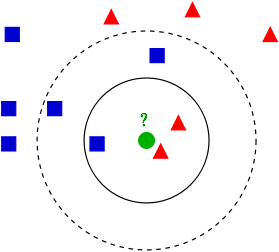
\includegraphics[width=0.3\textwidth]{Figures/knn.png}
\caption{Example of k-NN classification. The test sample (green circle) should be classified either to the first class of blue squares or the second class of red triangles. If k = 3 (solid line circle) it is assigned to the second class because there are two triangles and only 1 square inside the inner circle. If k = 5 (dashed line circle) it is assigned to the first class (3 squares vs. two triangles inside the outer circle) \cite{wikipedia_2017}.}
\label{fig:knn}
\end{figure}


\subsection{Implementation of a K-Nearest Neighbours Classifier}
 A K-nearest neighbours classifier was imported from the Sckit-learn package. The KNN classifier provided in this package provides many different parameters for modifying the algorithm.  It was decided to try to run classification with images resized to 50x50 pixels. The images also needed to be flattened. Flattening is a process of converting a multidimensional matrix into a vector. To flatten all pictures in the dataset, the height, weight and colour channels of images, were merged into one channel.

 To later test the classification performance, the dataset needed to be split into the separate training and testing datasets. The training dataset, as the name suggests, is used for an algorithm to learn the model and the test dataset is used only for evaluating the performance of the model. At first, it was decided, to use 70 percent of the randomly shuffled dataset as the training data and 30 percent as the test dataset (3168 training samples and 1359 test samples). That means that there were around 790 pictures for each of the four classes. After training a classifier, it was noticed that it performed rather poorly. Therefore it was decided to increase the number of images in the training dataset to 90 percent of the dataset. In this case, there were 4698 examples of training images and 522 examples of testing pictures.
 
It was tried to experiment with what K number of neighbours the classifier worked best, in order to improve the classification accuracy. After running the algorithm multiple times with different values of K, it was observed that the highest classification score was achieved with a K value = 18. However, the best accuracy score which was 36.28 percent was not an acceptable result, and it was necessary to improve the classifier.

 Images in the dataset were resized to the increased 100x100 pixels resolution, in order to test if larger image sizes would help the KNN classifier to perform better. When tested on k= 18 neighbours, the classifier showed the improved accuracy to 45.59 percent. To get a better understanding about how did the classifier perform a confusion matrix was plotted. From the confusion matrix \autoref{fig:k18}, it can be seen that Vanilla ice cream was classified correctly most often from the four classes. The accuracy of predicting it was 78.4 percent. The worst classified class was a salad which achieved only 0.02 percent accuracy.


\begin{figure}[h]
\centering
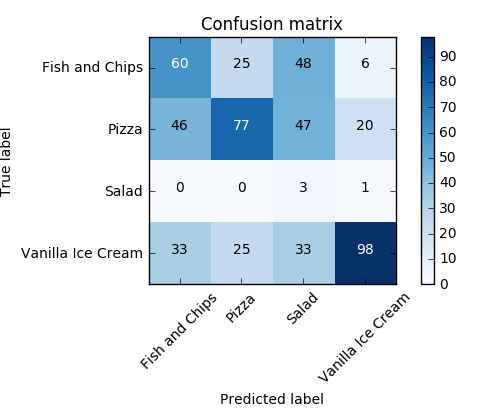
\includegraphics[width=0.5\textwidth]{Figures/conf_k-18.PNG}
\caption{Confusion Matrix of KNN classifier with k= 18}
\label{fig:k18}
\end{figure}




\subsection{Tuning of Hyperparameters}
Hyperparameters of a machine learning algorithm is a set of parameters that algorithm uses and that have to be specified while training the algorithm e.g.: K- amount of neighbours considered in the KNN classifier. Traditionally, hyperparameters were determined by humans, but the development of computing technology currently allows the use of various search techniques for better parameter optimisation.

There are two methods available for finding the best hyperparameters in the Sckit-learn package. These are an exhaustive grid search - GridSearchCV and a randomised grid search - RandomizedSearchCV.  The Exhaustive grid search tries to run an algorithm with all combinations of hyperparameters provided. The advantage of this approach is that the algorithm will always find the best combination of hyperparameters. However, exhaustive search algorithm has tried every single combination of hyperparameters before choosing the best set. It can be very computationally expensive and take a long time. Randomised search is usually able to find the set of parameters that can perform roughly equivalent than a grid search. The fact that that randomised optimisation could be a better optimisation technique was proven by Bergstra and Bengio who empirically and theoretically demonstrated that randomly chosen trials could be more efficient for hyper-parameter optimisation than trials on a grid \cite{bergstra2012random}.

 It was decided to optimise the following hyperparameters in the  K-nearest neighbours classifier: an amount of neighbours, a weight function that is used, and a distance function used. The number of neighbours considered was from k=1 to k=30. Weight function was either uniform meaning that during the classification the influence of all k neighbours is the same, or distance based, meaning that closer neighbours are more influential when the class of the target image is picked.  For the distance function, Manhattan and Euclidean distance were considered.


It was decided to try running the exhaustive grid search first to get the set of hyperparameters that works best for the classifier.Because hyperparameters sets are independent of each other, it was possible to run hyperparameter optimisation task in a parallel, using multiple cores of a CPU. Still, it took 30 minutes to run the exhaustive search on selected hyperparameters. It was found that the algorithm was most accurate with k = 8 neighbours, the Euclidean distance function, and uniform weights. Then, the algorithm was tested on the test dataset and classified it with 56.32 percent accuracy. More than 10 percent increase in accuracy was a considerable improvement from the previously achieved score.

From a plotted confusion matrix (\autoref{fig:k8}) it can be seen that the optimised KNN classifier was able to predict both pizza and ice cream classes very accurately. This fact is also confirmed in a precision, recall and f score table \autoref{table:1}. An average precision score of these two categories was around 0.8. However, the recall was lower - 0.53. The recall value was smallbecause the classifier misclassified a lot of images from different classes as pizza and vanilla ice cream.



\begin{figure}[h]
\centering
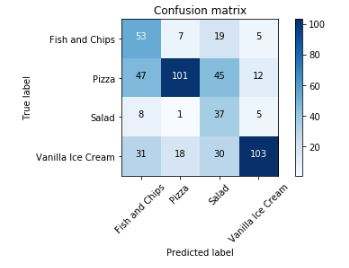
\includegraphics[width=0.6\textwidth]{Figures/knn.JPG}
\caption{Confusion Matrix of KNN classifier with k= 8, distance = Euclidean, weights= uniform}
\label{fig:k8}
\end{figure}

\begin{table}[h!]
\begin{center}
\begin{tabular}{ |c|c|c|c| } 
 \hline
 Class & precision &   recall & f1-score  \\ \hline
 Fish and Chips    &   0.38   &   0.63  &    0.48   \\
            Pizza   &    0.80  &    0.49 &     0.61 \\
            Salad    &   0.28  &    0.73  &    0.41  \\
Vanilla Ice Cream     &  0.82  &    0.57   &   0.67   \\ \hline
     Average     &  0.69   &   0.56    &  0.59  \\
 \hline
\end{tabular}
\caption{the precision, recall and f score of the best K-NN classifier}
\label{table:1}
\end{center}
\end{table}


   

\subsection{Results}

To conclude, with right optimisation of hyperparameters K- nearest neighbours classifier can classify images quite accurately. Pictures of a pizza and a vanilla ice cream class were classified much better compared to the images of the other two classes. The most misclassified class was a salad. The reason for that was the fact that there were images of various kinds of salad in the dataset. Because of that variance, salad class images were very scattered in the prediction space, and the classifier was unable to find the right neighbours.

The advantage of the classifier it that it can be trained in a very short time. However, it is was very slow when predicting the class of an unseen image. Because of that, different classification algorithms needed to be tried.
\iffalse
\section{Linear Classification}

Mapping image pixels to functions. 
F(x,W ) = W*x +b
Classifier can find which parts of the image is important for class of the image and which can be ignored (by setting some weights to low values and other to large)
If the dataset is unbalanced the bias for most likely class could be trained as higher than other

\section{Decision Trees}

\fi

\section{Support Vector Machine}

\subsection{Introduction to Support Vector Machine}

Support vector machine is one of the most influential machine learning algorithms \cite{boser1992training}. The algorithm searches for separators between classes that maximises the distance between them. Advantages of this classifier are that it can work very well on high dimensional data. Support vector machine tries to find a separating hyperplane for each class such that distances between separators and each class are as large as possible. A figure showing how a support vector machine chooses a hyperplane for separating two classes can be seen in \autoref{fig:svm}. Because this algorithm works well for a high dimensional data, it was decided to implement a classifier using SVM algorithm.

\begin{figure}[h]
\centering
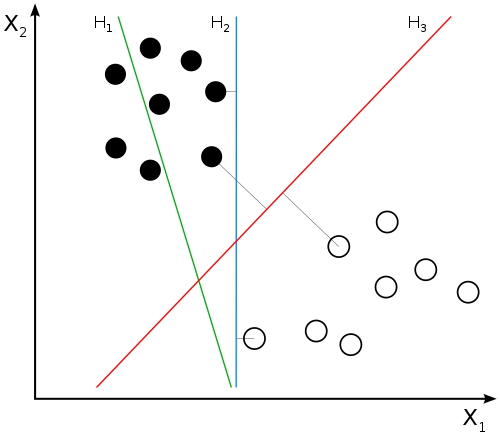
\includegraphics[width=0.5\textwidth]{Figures/svm.PNG}
\caption{Three hyperplanes are shown that could be used to split the data into two classes. H1 does not separate the classes. H2 does, but only with a small margin. H3 separates them with the maximum margin so it is selected as the class separator  \cite{wikipedia_2018}.}
\label{fig:svm}
\end{figure}


\subsection{Implementation of a SVM Classifier}

Support vector machine module was imported from the Sckit-learn package to start experimenting with it. To understand how the classifier works it was attempted to run the algorithm on our food data set resized to 100 x 100 pixels. At first, it was decided to try to run it with a default set of hyperparameters.

The training of the SVM classifier took around 60 minutes. When it was tested on test image data set, the accuracy achieved was only 25 percent.A confusion matrix was plotted \autoref{fig:svd},  to get a better understanding why the accuracy score was so low. The confusion matrix showed that for some reason the classifier classified all the test dataset as a salad. The hypothesis why the support vector machine classified all the data into the one class was that a decision surface that it learnt was too smooth.

The complexity of decision surface of SVM classifier is controlled by a  hyperparameter C and gamma. C parameter describes by how much the classifier should avoid misclassifying the training data. A little C makes the decision surface smooth but misclassifies more training data, while a high C aims at classifying all training examples correctly. \citep{hyper}. The Gamma parameter defines the influence that a single entity has on the decision boundary.  It was decided, to test what set of C and gamma could help to improve the classification accuracy.



\begin{figure}[h]
\centering
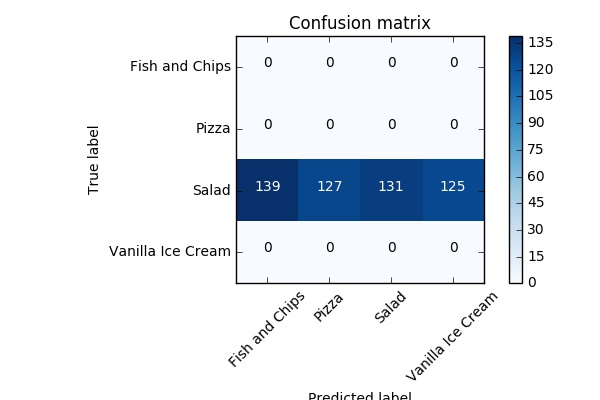
\includegraphics[width=0.5\textwidth]{Figures/svm_default.jpg}
\caption{Confusion Matrix of Support Vector Machine Classifier trained with default parameters}
\label{fig:svd}
\end{figure}


\subsection{Tuning of SVM Hyperparameters}

Because previous SVM model took a long time to train, it was decided to use only 10 percent of the training dataset to find best hyperparameters for this algorithm.

Firstly, it was chosen to increase the value of C. It was increased to the value of 10. With C=10 the algorithm trained on 10 percent of the dataset classified 26 percent of the test data correctly. After plotting the confusion matrix, it was observed that now the classifier predicted all classes \autoref{fig:svm_10_10} but it was very inaccurate in predicting.The C was increased to 100, but that did not improve the classifier.

Finally, the best set of C and gamma hyperparameters was found with randomised grid search. C values of  \(10, 100, 1000, 5000, 10000\) and gamma values  of \(0.0001, 0.0005, 0.001, 0.005, 0.01, 0.1\) were tried. Grid search found that C=10 and gamma = 0.0001 were the best set of parameters. It was reasonable that classifier worked best with the lowest value of gamma because images of food vary a lot and because of that a single image should not have too much influence on the separation lines between classes. It was tried to train the algorithm using a full train data set.

SVM was trained on the whole training dataset with C = 10 and gamma = 0.0001. Despite the fact that the hyperparameters were optimal, the accuracy of the classifier on the training set was only 25 percent. Plotted confusion matrix \autoref{fig:svm2} shown that the model still classified all test dataset as salad class. 

It was deducted that SVM algorithm was unable to classify the dataset correctly because a number of features considered when dividing the hyperplanes was too high. It was decided to use principal component analysis to reduce the number of features and test if that solves the problem.


\begin{figure}[h]
\centering
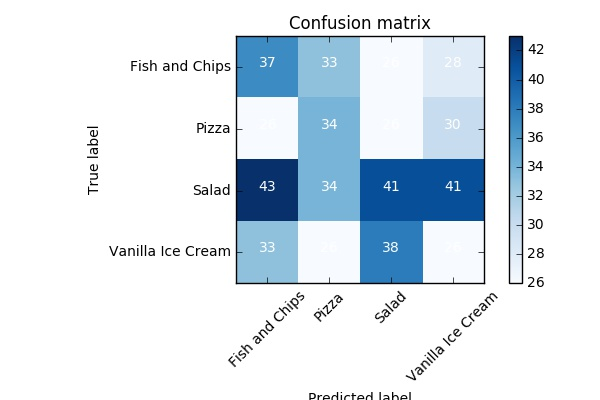
\includegraphics[width=0.5\textwidth]{Figures/svm_10_10.jpg}
\caption{Confusion Matrix of SVM trained with c = 10}
 \textit{Numbers in squares are: [37 33 26 28],
 [26 34 26 30],
 [43 34 41 41],
 [33 26 38 26]}
\label{fig:svm_10_10}
\end{figure}

\begin{figure}[h]
\centering
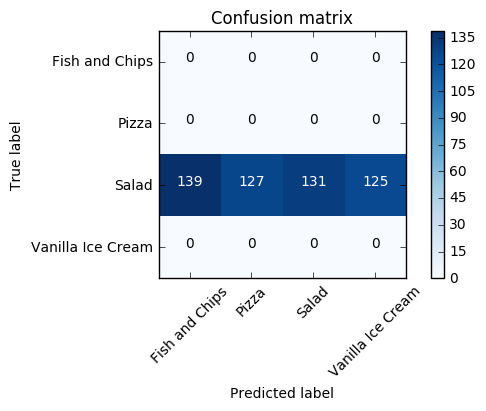
\includegraphics[width=0.5\textwidth]{Figures/svm2.png}
\caption{Confusion Matrix of SVM with C = 10 and gamma = 0.0001}
\label{fig:svd}
\end{figure}


\subsection{Reduction of  Dimentionality with Principal Component Analysis}
Principal component analysis is a simple, non-parametric method for extracting relevant information from confusing datasets \citep{pca}. It automatically detects strong patterns in the data and ignores the noise. Because food images contain many patterns and are usually noisy, PCA should be a good solution.  

The number of features was reduced from 30000 to 150 using this technique. Then, randomised grid search was performed to find the best C and gamma values for this support vector machine. 
It was found that algorithm classified the training data best with C = 1000 and gamma = 0.0001. After training, it was tried to classify the test dataset. The classifier achieved 60.73 percent accuracy which was the highest score compared to previously tried algorithms. Then a  confusion matrix and a classification report were plotted.From the confusion matrix displayed in \autoref{fig:conf_svm_pca}, it can be seen that all classes except the salad class were correctly predicted around 83 times. The most frequent misclassification was a fish and chips class misclassified as a pizza.From the classification report displayed in    \autoref{table:pca} it can be seen that a vanilla ice cream class had the highest precision and recall. The classifier predicted most of the ice cream pictures correctly. Because of that, it can be concluded that there was a distinct separator between vanilla ice cream class and other classes.

\begin{figure}[h]
\centering
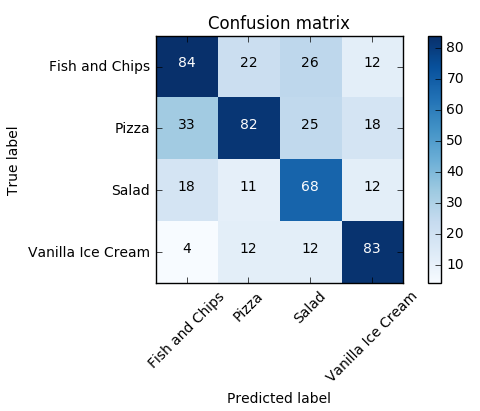
\includegraphics[width=0.5\textwidth]{Figures/conf_svm_pca.PNG}
\caption{Confusion Matrix of SVM classifier on the dataset reduced with PCA}
\label{fig:conf_svm_pca}
\end{figure}

\begin{table}[h!]
\begin{center}
\begin{tabular}{ |c|c|c|c| } 
 \hline
 Class & precision &   recall & f1-score  \\ 
 Fish and Chips    &   0.60    &  0.58    &  0.59 \\
            Pizza   &    0.65   &   0.52   &   0.58 \\
            Salad    &   0.65    &  0.52   &   0.58  \\
Vanilla Ice Cream     &   0.66    &  0.75   &   0.70   \\ \hline
     Average     &  0.61   &   0.61   &   0.61       \\
 \hline
\end{tabular}
\caption{A prescion, recall and f scores of the SVM classifier on the PCA reduced dataset}
\label{table:pca}
\end{center}
\end{table}

\section{Summary}

To conclude, the average test accuracy of 60 percent was achieved by both k-nearest neighbours and support vector machine with PCA models. This result proves that machine learning models can be used for classifying the food images. However, 60 percent accuracy is not good enough for using these models for real world applications such as dietary assessment. Therefore, other classification methods need to be explored. In \autoref{sec:intro} it was discussed that since 2012 deep learning has become a dominant method for image classification.  Deep learning methods are going to be presented in the following chapter. % Experiment 1

\chapter{Deep Learning approach for the Food Image Classification}
\lhead{\emph{Deep Learning approach for the Food Image Classification}}

In this chapter short introduction to deep learning is provided. Then the library used for building deep learning classifiers is described. Finally, deep learning models are constructed, and their performance is evaluated.


\section{Short Introduction to Deep Learning}

Deep learning is often regarded as an exciting and new technology. In reality, the field dates back to 1940s. The predecessor of deep learning was a linear classifier function. Linear models were designed to take a set of n input values \(x_1,...,x_n\) and associate them with an output \(y\). These models would learn a set of weights \(w_1,...,w_n \) and compute their output \(f(x,w)=x_1 w_1+...+x_n w_n\) \citep{Goodfellow-et-al-2017}. This function was motivated by our understanding of how neurons work in living organisms. 

The same function is used in today's deep neural networks. A deep neural network contains a set of linear functions connected in a way where the output of the previous function is the input to the next function. The result of \(f(x,w)\) is then passed through the non-linear activation function to make the result non-linear. The most commonly used activation function today is a Rectified linear unit (ReLU). ReLu can be mathematically described as \(f(x)=max(0,x)\). It always outputs 0 for values less than 0 and \(x\) for values greater than 0. Illustration of this is shown in \autoref{fig:relu}. Neural networks using this function usually converge faster than networks using a different activation function \citep{relu}.

\begin{figure}[h]
\centering
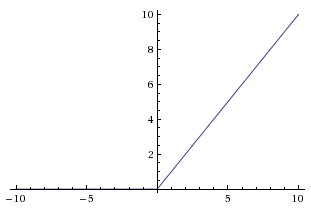
\includegraphics[width=0.5\textwidth]{Figures/relu.jpeg}
\caption{The ReLU Activation Function \citep{231nn}}
\label{fig:relu}
\end{figure}


\section{Introduction to TensorFlow}

TensorFlow is an interface for expressing machine learning algorithms and an implementation for executing such algorithms. A computation expressed using TensorFlow can be executed with little or no change on a wide variety of systems, ranging from mobile devices such as phones and tablets up to large-scale distributed systems and thousands of computational devices such as GPU cards \cite{abadi2016tensorflow}. The system is flexible and can be used to express a wide variety of algorithms for deep neural network models. Computations in TensorFlow are described in a directed graph. First, all listed operations are added to the graph. Then a TensorFlow session is called which executes the operations in the graph. An example of a TensorFlow program that adds two scalars and computes the result can be seen in \autoref{fig:sess}. Executing tf.add(5, 5) creates a node in the computational graph with 5 and 5 as the input values. The result of the add operation is only computed when a TensorFlow session is created. 

It was decided to use TensorFlow to construct deep neural network models for food image classification because this library is fast and efficient. It is used by many deep learning researchers. However, because TensorFlow was created primary for conducting deep learning research, algorithms provided in this library are low level and require additional implementations to make them work on a particular dataset.

Because of the complexity and a low-level implementation, it was a very challenging task to learn and understand how to use TensorFlow correctly.  To get familiar with TensorFlow, it was firstly tried to implement deep learning models for the default datasets provided in the TensorFlow library. After spending a significant amount of time studying deep learning methods and writing implementations of deep learning algorithms, steps needed to train a neural network model with TensorFlow were eventually discovered. However, before training the models the dataset, needed to be transformed into a format supported by TensorFlow. 

\begin{figure}[h]
\centering
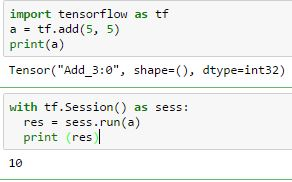
\includegraphics[width=0.5\textwidth]{Figures/4/sess.jpg}
\caption{TensorFlow Program that Adds two Scalars}
\label{fig:sess}
\end{figure}

\section{Transformation of the Dataset For Using It with TensorFlow}

Before using the food image dataset, additional preprocessing techniques needed to be applied. The class labels of this dataset were represented by strings e.g.: "Pizza". Non-numerical class names cannot be used when computing a distance function and other functions that are used in machine learning. Therefore, class labels had to be transformed using the one-hot encoding. One-hot encoding converts every class name into a vector which has the length equal to the number of categories. For every class, one element in a vector is set to one while other elements are set to zeros. The previously used Sckit-learn library encoded the labels automatically, but in TensorFlow this task has to be done manually.

To one-hot encode, the labels of the dataset were first transformed into numeric values from 1 to 4. After that, a vector equal to the number of classes was created, and numeric values were converted to one hot encoded values (\autoref{table:oh}). After the transforming the labels of the dataset, it was possible to use it for training deep neural networks with TensorFlow.


\begin{table}[h]
\begin{center}
\begin{tabular}{ |c|c|c| } 
 \hline
 Label &   Numeric label & One-hot Encoded label  \\   \hline
 Fish and Chips    &   1  &   [0, 0, 0,1]  \\
            Pizza   &   2 &    [0, 0, 1,0]    \\
            Salad    &   3 &    [0, 1, 0,0]    \\
Vanilla Ice Cream     &  4  &   [1, 0, 0,0]    \\ 
 \hline
\end{tabular}
\caption{One-Hot Encoding for the Dataset}
\label{table:oh}
\end{center}
\end{table}


\section{Linear Classifier in TensorFlow}
It was decided to construct linear classifier as a first TensorFlow classification model. This classifier was chosen because it is very simple compared to other neural network models. Furthermore, a linear classifier is a building block of every deep learning model, so it was  important to understand it well before building more complex classification models

\subsection{Introduction to a Linear Classifier}
 Linear classifier can be described as a function \(y = w\times X\). In a case of image classification, \(y\) is a class of an image, \(X\) is a vector of pixels of an image and  \(w\) is a vector of weights that are associated with each pixel. The fact that each pixel has a separate weight associated with it allows this classifier to learn the important areas of pictures in each class automatically. The classifier can calculate which parts of the image have a large influence when classifying an image and make the weights of these pixels large. The weight of pixels that have no or tiny impact to the class of a picture can be set to values that are close to zero.

\subsection{Training  of  the Linear Classifier}
To begin training the model, the weights were initialized with random values from a generated normal distribution with 0.01 standard deviation. After the weights had been initialized, the classifier tried to classify the data with the initialized weights. Then, the error function was calculated, and the weights were updated to the values that decreased the error function. The update rate value was controlled by a learning rate. The learning rate that was used to train this model was 0.005. To perform the weight optimisation a gradient descent and Adam optimizer was tried.

Gradient descent is an algorithm that tries to minimise the training lost, and the Adam optimizer is a gradient descent optimisation algorithm. Adam works well in practice and compares favourably to other optimisation methods \citep{adam}. The advantage of Adam optimizer is that it can start optimising weights with a high learning rate and then automatically decrease it as the algorithm continues to train. Consequently, Adam optimizer can find the optimal weights faster than a gradient descent.

It was possible to train the optimisation algorithm on the full dataset or use batch optimisation. For using batch optimisation,  the training dataset has to be split into batches of equal size. Then, optimisation algorithm runs on the one batch of the dataset, updates the weights of the full dataset, and uses a different batch for optimising the weights again. The advantage of using a full dataset for weights optimisation is that more data usually leads to a better weight optimisation. However, running this algorithm can take a very long time. Usually, batch optimisation is faster and can achieve similar results.

To do a batch optimisation, the food image dataset was split into 54 batches containing 87 food images each. From all trained linear classification models the classifier that used the Adam Optimizer with 0.05 learning rate and the batch optimisation performed the best. It achieved 51.53 percent accuracy. A table of classifiers tested and their performance can be seen in \autoref{table:linear}. To be able to use these models without having to retrain them, they were saved to a disk.


\subsection{Results}
From the results table, it can be observed that optimisation on the full dataset performed very poorly compared to the batch optimisation method.  This happened because the weights on batch optimisation were updated 56 times more often. It can also be observed that Adam Optimizer was a better optimisation algorithm than a gradient descent. It performed 7.09 percent better. 

To conclude, despite the fact that a linear classifier is such a simple algorithm, it was possible to optimise it to classify the images with a reasonable accuracy.

\begin{table}[h]
\begin{center}
\begin{tabular}{ |c|c|c|c| } 
 \hline
 Learning Rate &   Optimization Function & Batch Size & Classification Accuracy \\   \hline
0.005    &   Adam   &  85  & 51.53\% \\
0.005    &   Adam &  full dataset  & 26.00\% \\
0.005    &   Gradient Descent   &  85  & 44.44\% \\ 
 \hline
\end{tabular}
\caption{The Influence of the Hyperparameters to the Accuracy of the Linear Classifier }
\label{table:linear}
\end{center}
\end{table}

\section{Multi-layer Neural Network in TensorFlow}

After building a linear classifier, it was decided to expand it to build a deep neural network, which could learn a better representation of the data. The structure of the model was designed in the following way: 30,000 neurons in the input layer, two hidden layers containing 256 neurons each and a final layer containing four neurons that map to the four image classes. A ReLu activation function was used in hidden layers to introduce a non-linearity to the network (\autoref{fig:3lay}). 

\begin{figure}[h]
\centering
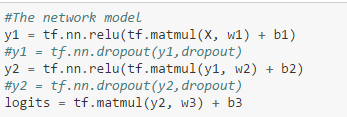
\includegraphics[width=0.5\textwidth]{Figures/3layer.PNG}
\caption{Snippet of the 3 Layer Network Model}
\label{fig:3lay}
\end{figure}


After starting to train the model, it was observed that after a couple of training epochs the training accuracy stopped improving and stayed the same during all the duration of training. When tested on the test dataset, the classifier classified the food images with only 24 percent accuracy, which was even worse than a random guessing. It was, though that the problem was with the learning rate being too high. However, decreasing the learning rate did not solve the problem. Then, it was tried to change the structure of the network by changing the number of layers in the network and number of neurons in each layer, but modifying the structure did not solve the problem either. Various sets of different hyper-parameters were tried to fix the network, but nothing seemed to work. It was finally noticed that the problem was caused by a wrong activation function used in a final layer. TensorFlow library did not provide any warning about the error making it hard to detect the problem. 

After fixing the error, the classifier was trained using the Adam optimizer with a learning rate of 0.0001. When tested this classifier achieved 56.32 percent accuracy. It was noticed that during the training of this classifier, the cost function decreased slowly. Because of that, it was decided to increase the learning rate to 0.001. However, this learning rate seemed to be too large, and the classifier accuracy decreased to 47.50 percent. Then 0.0005 learning rate was used. The network trained with this learning rate classified the test data with 54.02 percent accuracy. After experimenting the different learning rates, it was concluded that  0.0001 was the optimal learning rate for this neural network.

Finally, it was decided to try to increase the number of layers in this neural network. It was expected that a deeper network would be able to learn a better representation of the dataset. Five layer neural network model with four hidden layers that have 256, 256,256 and 128 neurons classified the test dataset with 56.32 accuracy. This accuracy was the same as achieved with a three-layer neural network. It was tried to improve accuracy by changing the number of neurons in different layers. The neural network that had fewer neurons in the final hidden layer performed a bit better, but no other significant improvements for classifying the test dataset were noticed. A full table of multilayer classifiers that were trained and their performance can be seen in \autoref{table:multi}.

\begin{table}[h]
\begin{center}
 %\setlength\tabcolsep{2pt}
\begin{tabular}{ |c|c|c|c| }
\hline
 Learning Rate &   Number of layers &  Neurons in each layer& Accuracy \\   \hline
0.0001    &   3  &  256, 256, 4  & 56.32\% \\
0.0005    &   3  &  256, 256, 4  & 54.02\% \\
0.001    &   3  &  256, 256, 4  & 47.50\% \\
0.0001    &   5  &  256, 256, 256, 128, 4  & 56.32\% \\
0.0001    &   5  &  256, 256, 256, 64, 4 & 58.81\% \\  
 \hline
\end{tabular}
\caption{The Influence of the Hyperparameters to the Accuracy of the Multi-layer Neural Network  }
\label{table:multi}
\end{center}
\end{table}

\subsection{Results}

To conclude, a multi-layer neural network performed a little better than a linear classifier. The best neural network design was a five layer neural network with 30,000 input neurons, 256 neurons in the each hidden layer and four neurons in the output layer. When trained with a 0.0001 learning rate, it achieved 58.81 percent accuracy on the test dataset. The achieved accuracy was  7.28 percent better than the accuracy of the best linear model. 

However, the design process of multi-layer neural networks was much more complicated. There are no formal definitions that state how many layers a network should have or how many neurons should be in these layers. Therefore, a collection of experiments is needed to find an optimal network design. Training of multi-layer neural networks is also more computationally expensive and takes a longer time.

\section{Convolutional Neural Networks in TensorFlow}

\subsection{Introduction to Convolutional Neural Networks }

A convolutional neural network (CNN) was introduced in 1989 to solve a problem of classifying handwritten digits by \cite{lecun}.
A typical layer of a convolutional neural network consists of three stages. In the first step, the layer performs several convolutions in parallel to produce a set of linear activations. In the second stage, each linear activation is passed trough a nonlinear activation function, such as rectified linear activation function. In the third stage, a pooling function is used to replace the output of a particular location in the network with a summary statistic of the nearby outputs \citep{Goodfellow-et-al-2017}. The most commonly used pooling operation in convolutional neural networks is max pooling \citep{max}. It converts the rectangular area of the output into one value representing the maximum value in that output (\autoref{fig:max}). For training a convolutional neural network, only preprocessing that has to be done is converting each image to the same size.

Convolutional neural networks work by extracting the features from images automatically. This approach tends to work better than a manual feature engineering.

\begin{figure}[h]
\centering
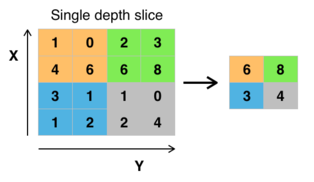
\includegraphics[width=0.5\textwidth]{Figures/4/Max_pooling.png}
\caption{Illustration of the Max Pooling}\medskip The function outputs a maximum output in every 2 by 2 square \citep{wiki:Convolutional}
\label{fig:max}
\end{figure}
 

\subsection{Implementation of a Convolutional Neural Network}

Training a convolutional neural network requires sufficient amount of computing power. Therefore,  GPU cards are used for training convolutional neural networks. Since a computing device with separate GPU unit was not available, it was decided to focus on smaller CNN architectures that could be trained on a CPU.

It was chosen to design a convolutional neural network with three convolutional layers and one fully connected layer. First, convolutional layer applies one by one convolution to the input picture and creates four convolution images. These convolution images are then passed through an activation function at outputs of this function are passed into a second convolutional layer. Besides convolution, a max pooling operation is also applied in the second and third layers of the network. The final convolutional layer outputs twelve seven by seven convolutional images. These images are passed into the fully connected layer, and finally, the class of a picture is calculated in the final layer \autoref{fig:con_mod}



\begin{figure}[h]
\centering
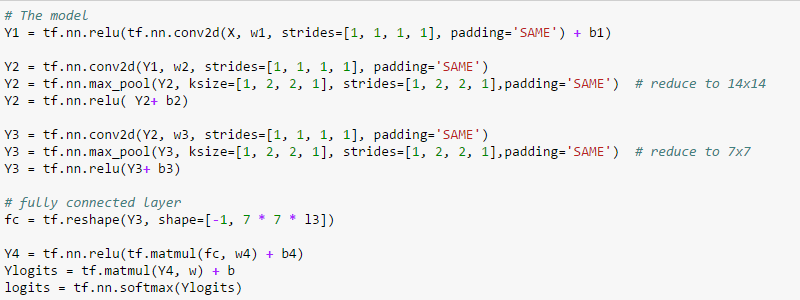
\includegraphics[width=0.5\textwidth]{Figures/4/conv.PNG}
\caption{The Convolutional Neural Network Model in TensorFlow}
\label{fig:con_mod}
\end{figure}

Firstly, the images of the dataset were resized to 26 by 26 pixels to reduce the dimensionality of the data.
It was unknown how long it would take to train the network, so it was decided to reduce the dimensionality even further by converting images to greyscale.

Then, a convolutional neural network was trained for 100 epochs. The best learning rate that was used in the deep learning network (0.0001) was too small for the convolutional network. The learning rate was gradually increased, and it was observed that learning rate 0.003 suited the network best. The network with this learning rate achieved 100 percent accuracy on the training dataset in 68 epochs. Despite the fact that the result looked very impressive, it was known that convolutional neural networks tend to overfit the data. That means that they learn to classify the training dataset very accurately but do not classify the test dataset well. Therefore, the classifier was tested on the test dataset. It achieved 38.12 percent accuracy, which was not a  good score.

The algorithm was modified to accept RGB images to test whether colour channels have an influence on the classification accuracy. After the network had been trained, it was observed that it achieved 47.51 percent accuracy on the test dataset. More than 9 percent increase in accuracy showed that colour is a major component for a food image classification and should be kept if possible. The architecture of both convolutional neural networks trained is shown in \autoref{table:convi}. The picture illustrating different layers in this network is shown in \autoref{fig:conv2}.

\begin{table}[h]
\begin{center}
 %\setlength\tabcolsep{2pt}
\begin{tabular}{ |c|c|c|c|c| }
\hline
 Input image&Learning Rate &   Number of layers & Architecture & Accuracy \\   \hline
28x28x1 & 0.003   &   5  &  3 x conv, fc, o  & 38.12\% \\
28x28x3 & 0.003   &   5  &  3 x conv, fc, o  & 47.50\% \\
 \hline
\end{tabular}
\caption{The First two Convolutional Models Tried}

\label{table:convi}
\medskip
\textit{ conv - convolutional layer, fc - fully connected layer, o - output layer}
\end{center}
\end{table}


\begin{figure}[h]
\centering
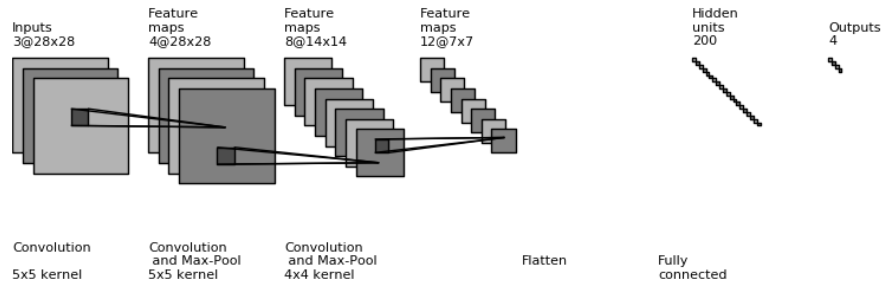
\includegraphics[width=0.8\textwidth]{Figures/4/conv_diagram.PNG}
\caption{Layer Diagram  of the  Convolutional Neural Network }
\label{fig:conv2}
\end{figure}


\subsection{Improving the Convolutional Neural Network}

Since both classifiers achieved a hundred percent accuracy on the training dataset and performed poorly on the test dataset, it was clear that the classifiers were overfitting the data. It was decided to add dropout layers to the network, to fix this problem. Dropout is a method used to prevent neural networks from overfitting. The key idea is to randomly drop units (along with their connections) from the neural network during training \citep{dropout}. Dropout function prevents neurons from co-adapting too much. 

A 50 percent dropout rate was added to the every layer in the network. The Introduced drop layer helped to prevent the network from overfitting. However, because of the high dropout ratio, the network was unable to optimise the weights, and it classified worse than previously trained models. The learning rate of the network was increased, to solve this problem. However, this solution did not work. Larger step size caused the optimisation algorithm to keep overshooting the minimum. The other tried solution was increasing the probability to keep neuron connections to 80 percent. It improved the classification accuracy for both grayscale and RGB image classification, but the improvement was only marginal (49.04 percent accuracy for RGB test data and 40 percent accuracy for the grayscale image classifier). Lastly, a network that kept 90 percent of the neuron connections was built, but it decreased the accuracy of the model achieved on the test dataset. It was concluded that learning rate 0.003 and 20 percent dropout probability were the best set of hyperparameters for this network. Because there were no more hyperparameters that could be further optimised it was decided to build a neural network that could handle larger size images.


\subsection{Designing Convolutional Neural Network  for Larger Images}

It was expected that larger image size would lead to a better accuracy score when performing image classification. Larger image sizes allow more information to be preserved in pictures. The network was redesigned to take 56x56x3 pictures as an input. One more convolutional and a max-pooling layer were also introduced to the architecture of the network. Then, it was tried to find the optimal learning rate. The network was trained with 0.003 learning rate and a 20 percent dropout probability for 30 epochs. It was noticed that learning rate, which worked very well for the previous neural network, was too high for this network. Because of that, the gradient optimisation algorithm kept overshooting the minimum. Therefore, the training accuracy and loss stayed the same during the training of the model. The learning rate was gradually lowered, to find the optimal learning rate.  It was found that the largest learning rate that could be used was 0.0015. With this learning rate, the algorithm was able to learn the optimal weights. When tested, it achieved 60.72 percent test accuracy. It was observed that after 30 epochs the optimisation algorithm was still improving. Therefore,  the number of epochs were increased to 100.  That allow the weights to be optimised more precisely. After testing the model on the test dataset, it was observed that the accuracy increased to 62.26 percent.

Finally, the architecture of dropout layers was modified, to test whether it could improve the performance of the classifier. In the previous model, dropout was used in every layer except the fully connected one. The dropout was added to the fully connected layer too. However, after adding the dropout, the learning rate value of 0.0015 became too large. After decreasing the value of the learning rate to 0.001, it became possible to train the network. The trained network with 20 percent drop probability reached 69.34 percent accuracy, and a trained network with 30 percent drop probability reached 63.98. Therefore, 20 percent was a better drop rate in both approaches. It was also tried to modify the model to use dropout only in a fully connected layer. Because only one dropout layer was used, the dropout probability was increased to 50 percent. The network was trained with a 0.001 learning rate. However, training accuracy of the model improved very slowly. Therefore, the learning rate was increased, until its optimal value of 0.002 was found. The trained model was tested on the test data set. The accuracy of the model on the test dataset was 51.54 percent. The table of CNN networks that were constructed for 56x56x3 images can be seen in \autoref{table:53x53}.


\begin{table}[h]
\begin{center}
\begin{tabular}{ |c|c|p{3.3 cm}|p{2 cm}|c|c|} 
 \hline
 Learning Rate & Drop probability & Network layers with drop &Training Epochs&Accuracy \\   \hline
0.001   &   20\%  & Every except fully  connected  & 30 & 57.08\% \\ \hline
0.0015    &   20\%   &  Every  except fully connected  & 30  & 60.72\% \\ \hline
0.0015    &   20\%   &  Every  except fully connected  & 100  & 62.26\% \\ \hline
0.001    &   30\%   &  Every  & 100  & 63.98\% \\ \hline
0.001    &   20\%   &  Every  & 100  & 69.34\% \\ \hline
0.002    &   50\%   &  Fully connected& 100  & 51.54\% \\  \hline
\end{tabular}
\caption{Configurations for Convolutional Neural Networks tried with 56x56x3 Pictures}
\label{table:53x53}
\end{center}
\end{table}



\section{Transfer Learning Technique}

\subsection{What is Transfer Learning}

Currently, all state of the art image classifiers are large convolutional neural networks.  For training these networks, large GPU clusters were used.  It usually takes multiple weeks to train these models. For example,  the Google Inception v3 network was trained on a cluster of  50 computers with  NVidia Kepler GPUs \citep{incept}. It is impossible to train this network using only one computer because it has millions of parameters that require a massive amount of memory and computation power. The only way how this network could be retrained for a different dataset on a regular computer is by using a transfer learning approach. 

Transfer learning is a technique that shortcuts a lot of this work by taking a fully-trained model for a set of categories like ImageNet and retrains it from the existing weights for new classes \citep{tensorflow}. Usually,  to save time, only the two final layers of a neural network are retrained. The reason why retraining only the last two layers is sufficient is that convolutional layers tend to activate to patterns of different shapes, colours and edges. Such patterns appear not to be distinct to a particular dataset or task, but can be applicable to many datasets and tasks \citep{transfer}.

It was chosen to retrain the Google Inception v3 model. A python script for loading and retraining this model is publicly available in the Tensorflow's Github repository \citep{gitretrain}. The script provides the ability to tweak hyperparameters such as the learning rate, number of training epochs and a batch size. 


\begin{figure}[h]
\centering
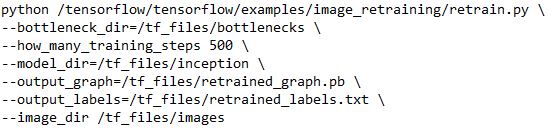
\includegraphics[width=0.5\textwidth]{Figures/4/term.PNG}
\caption{Command Used to Retrain the Inception v3 Model}
\label{fig:retrain}
\end{figure}

\subsection{ Retraining the Inception v3 Model}

The classifier was retrained with a learning rate = 0.01, a number of epochs = 500 , and a batch size = 100. The script split the dataset to use 80 percent of it as a training set, 10 percent of it as a testing set used to test the classifier after each epoch and the last 10 percent as a validation dataset used to test the trained model. The terminal command that was used to run the retrain.py can be seen in \autoref{fig:retrain}.

When retrain.py was executed, it calculated bottlenecks for all the images in the dataset. A bottleneck is a term used for naming the layer just before the final output layer that does the classification. Calculation of bottlenecks took a significant amount of time. The script saved the calculated bottlenecks to the disk, so this task was only needed to run once.

After the calculation of the bottlenecks. The weights of the penultimate and final layers were set, and optimisation of weights in these layers began. The training progress of the classifier was shown in the terminal (\autoref{fig:retrain}). It was observed that just after ten epochs the classifier reached 96 percent accuracy.  After running the weight optimisation algorithm for 500 iterations, the final trained model achieved 98.2 percent accuracy when tested on 507 validation samples. That meant that the classifier was able to classify 98 from 100 pictures of unseen food correctly.  This accuracy is much higher than accuracies achieved by every other classifier.

To obtain a better understanding how can this classifier perform on the real-world data 5 example pictures for each class were downloaded.These images were a had picked examples of each class. The python script that loads the learnt model from disk, and feeds classifier with images from the given folder was written. After running the classification on 20 accumulated images, one classification error was detected. The classifier classified a picture of deep pan pizza (\autoref{fig:miss}) as fish and chips. It was expected that this example might get misclassified because there were no deep pan pizzas in a training dataset. The smooth structure of a crust of the pizza can also resemble a battered fish. 


\begin{figure}[h]
\centering
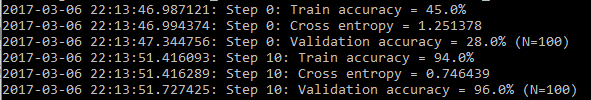
\includegraphics[width=0.5\textwidth]{Figures/4/term-train.PNG}
\caption{Retraining  of the Classifier, 96 Percent Accuracy was Reached in  10 Epochs}
\label{fig:retrain-2}
\end{figure}

\begin{figure}[h]
\centering
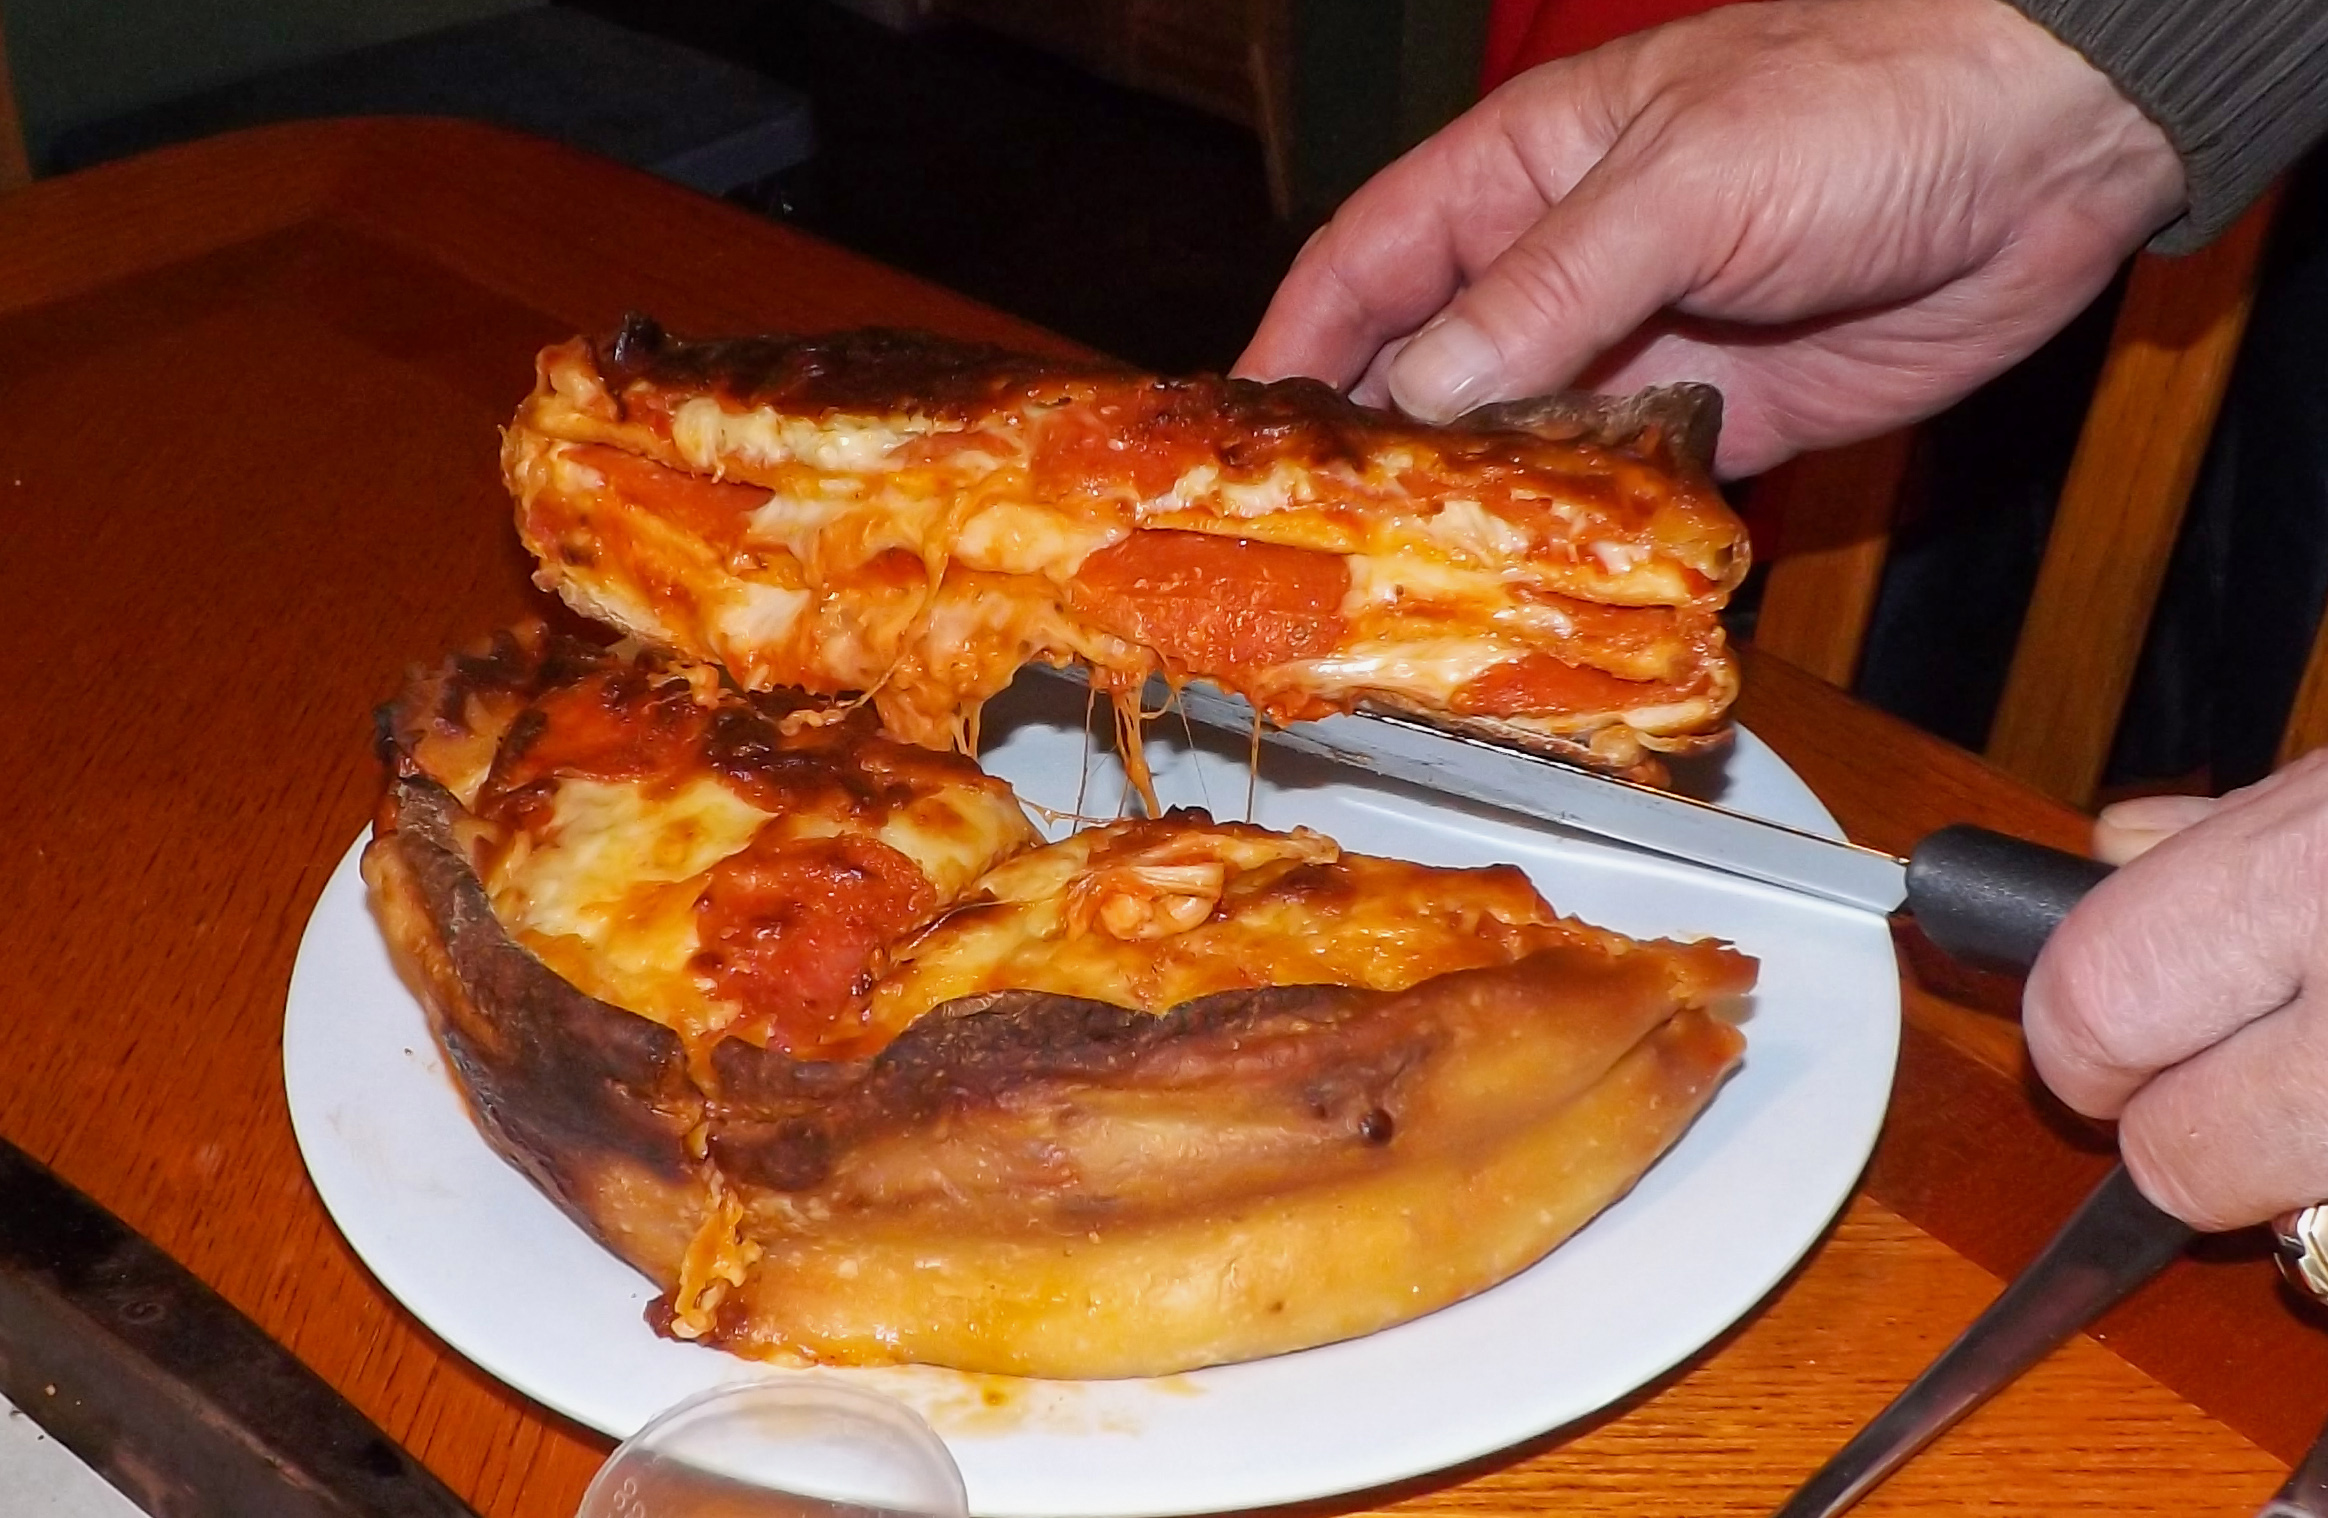
\includegraphics[width=0.5\textwidth]{Figures/4/4.jpg}
\caption{Deep Pan Pizza that was Missclassified as a Fish}
\label{fig:miss}
\end{figure}




\section{Summary}

To conclude, it can be clearly seen that deep learning networks on average performed much better than a standard machine learning models. The accuracy achieved by a transfer learning model was very high. The model could be used in practice because the error rate is very low.

However, finding the optimal parameters for the deep neural network models is a much harder task. It requires an excessive effort to design an architecture of a neural network. What structure of the network will work on a particular task,  cannot be known beforehand. Therefore, many architectures have to be tried to find a suitable architecture. Even then it is unknown if the chosen architecture is actually the best because the configuration space is gigantic.

In the next chapter, the results of all classification methods are compared. % Experiment 2


\chapter{Results}
\lhead{\emph{Results}}
In this chapter, the results of each classification method are going to be compared. Then, advantages and disadvantage of these methods are going to be discussed.

\section{Comparison of Accuracy Scores}

Results of the best classification model of each method tried are shown in  \autoref{table:all}. From this table, it can be seen that transfer learning is the best classification method with 98.20 percent accuracy. The convolutional neural network is at the second place with 69.34 percent accuracy.  The difference in accuracy score between other classification methods is not that marginal. Linear classifier achieved the lowest accuracy score of 51.53 percent while support vector machine model achieved accuracy score of 60.73 percent. 

\begin{table}[h]
\begin{center}
\begin{tabular}{ |c|c| } 
 \hline
Method &  Classification Accuracy \\   \hline
KNN    &  56.32\% \\
SVM with PCA   & 60.73\% \\
Linear   &    51.53\%  \\
3 Layer    &   54.02\% \\
5 Layer    &  58.81\% \\
CNN & 69.34\% \\
Transfer  &  98.20\% \\

 \hline
\end{tabular}
\caption{Best classifiers of each method}
\label{table:all}
\end{center}
\end{table}


\section{Comparison  of time complexity of the classifiers}
There are three kinds of time complexities that can be considered for evaluating machine learning classifiers. The first one is a build-time complexity - how long does it take to build the classification model. The second one is a training complexity - the amount that it takes to train the classification model. The final one is a runtime complexity - how long does the classifier take to tell a class of an item. 

The K-nearest neighbours classifier was simple to build.  It only required a hyper-parameter optimisation which was rather quick. The training of the algorithm was also fast because to train this algorithm the only required task is saving the dataset to the memory. However, the runtime performance of this classifier was not great. During the runtime, this algorithm calculates a distance between an item that class is needed to be predicted and every other element in the dataset. Later these distances are compared to find the K closest distances. That is a very computationally expensive task.

It was a much more difficult task to get Support Vector Machine Algorithm to work. Despite the fact, that the algorithm was designed to work on a high dimensional data,  the food image dataset was too complex for it. The only way to use this algorithm was by firstly applying the PCA to the dataset. Therefore, building this model required a significant amount of experimentation and took a much longer time, before actual results were seen. It took a very long time to train the support vector machine. Prediction time was faster than the prediction time of the KNN classifier but was not instantaneous.

The Linear classifier did not take much time to create because it is a very simple classification model. Training of this algorithm was fast because the only things calculated were a matrix product of training images and weights, and ran an optimisation algorithm. Prediction time was almost immediate.

Deep neural network required much more experimentation, to make it work. Training of the algorithm took a long time, but the prediction was almost as fast as the linear classification model.

Convolutional neural network required, even more, engineering work. Some CNN models architectures that were tried had a very low classification accuracy. Various models had to be tested, to finally find the architecture that was working.  Training of the algorithm took the longest amount of time from all the algorithms implemented. However, the classifier was able to predict the classes of new pictures very quickly.

The transfer learning technique was simple because the model with a python script was provided by Google. In a case where one has to write a script that retrains the final layer,  it can be a very hard task. The calculation of the bottlenecks took a long time. Therefore a training complexity of this algorithm was high.  However, for classifying the images, this algorithm took the same time as other neural networks.

To conclude, the algorithm that took the least time to built was KNN. The most time was spent deep neural network models because finding an appropriate network architecture was a very hard task. The classification algorithm that took the least time to train was KNN. For fastest prediction times, the linear classifier was the best option.

\section{Possible improvements and limitations of classification models}

The KNN classifier, the SVM,  and the linear classifier model can not be considerably improved.  Hyperparameters of these algorithms were optimised. Therefore, the only possibility for improving them is training these models on a more powerful machine with a larger image size.

In contrast,  the accuracy of the deep neural network and the convolutional neural network can still be considerably improved.It can be done by adding more layers or modifying the structure. The number of ways that these networks can be configured is infinite. 
That makes optimisation possible but hard task. It is unknown what structure is needed.

That is the main limitation of neural networks that was observed in this project. A person building deep or convolutional neural network has to make a lot of decisions that directly impact the performance of the network. Choosing the number of layers and the number of neurons in each layer is a challenging task. Furthermore, activation function and weight optimisation function needed to be selected too.

\section{Summary}

To conclude transfer learning achieved the highest classification score. However, this model was not built from the ground up. The best model that was built was the convolutional neural network which achieved 69.34 \% accuracy.  It was also discussed that deep neural network models are very hard to build and take much longer time to train when compared to other classification methods. In the next chapter, the conclusions of the work are going to be deducted.
 %Results

\chapter{Conclusions}
\lhead{\emph{Conclusions}}



The Objectives of the project were to practically understand machine learning algorithms that can be used for classifying images. To accomplish this task,  a suitable food image dataset was found and food pictures were preprocessed. Then, image classifiers using various machine learning algorithms were built.  Finally, these classifiers were trained on the accumulated dataset and their performances were evaluated.

\section{Lessons Learnt}

During the progress of this project, it was gradually discovered why image classification is such a hard problem.  The problem that algorithms in image recognition task face is that images are very dynamic and are susceptible to different kind of variations. It was practically observed that machine learning algorithms that are successfully used in practice for tasks such as spam detection, credit card fraud detection and other tasks were unable to classify images with a sufficient accuracy.  It was also observed that machine learning algorithms take a very long time to train. This is the main barrier for using machine learning techniques for vision. Overall, the project was successful. A framework for converting pictures to the dataset of images was built. Then,  machine learning classifiers that used different classification algorithms were developed and their performance was systematically evaluated.

\section{Limitations}
The main limitation of the project was that machine learning algorithms take a very long time to train. Images are very high dimensional data, and an enormous amount of the computing power is required to train a good machine learning model for image classification. Therefore, this project was limited to using only four image classes. These four classes are not able to represent all types of food that is eaten by people.

The second limitation that was faced during this project was that it was not possible to explore larger deep learning networks on the hardware setup used. Therefore, a maximum accuracy score of the deep neural network and the convolutional neural network could not be reached. With deeper architectures of neural networks, it would be plausible to achieve better accuracy scores.

\section{Future Work}

To extend this project, one classification method should be explored more thoroughly and a classifier that distinguishes between a greater amount of food classes should be built using this model.   A convolutional neural network would be the most promising model to explore further because it achieved a high accuracy score. Also, researchers have proven that a convolutional neural network is the best method that can be used for image classification. Furthermore, there here has been few studies about  a food classification with convolutional neural networks.  A good number of classes for a new model would be around 100 types of most popular dishes.  Because of the increased complexity, a GPU cluster will be needed to train this model. If this new model achieved the high accuracy rate, it would be possible to use this model in dietary assessment applications.


 % Conclusion


%% ----------------------------------------------------------------
% Now begin the Appendices, including them as separate files

\addtocontents{toc}{\vspace{2em}} % Add a gap in the Contents, for aesthetics

\appendix % Cue to tell LaTeX that the following 'chapters' are Appendices

\chapter{A Computer System used for the project}

Performance of Machine Learning algorithms can be directly mapped to a computing power of a computer system used. With more computing power it is possible to train algorithms using more training data or with using a bigger set of features. Because of that it is important to show the parameters and limitations of the computer system used.

CPU: Intel(R) Core(TM) i5-4210U CPU @ 1.70GHz

	Maximum speed:	2.40 GHz
	Cores:	2
	Logical processors:	4
	L1 cache:	128 KB
	L2 cache:	512 KB
	L3 cache:	3.0 MB


Memory: 8.0 GB DDR3, frequency:	1600 MHz

Disk: Samsung SSD 850 EVO 500GB
	% Appendix Title

%\input{Appendices/AppendixB} % Appendix Title

%\input{Appendices/AppendixC} % Appendix Title

\addtocontents{toc}{\vspace{2em}}  % Add a gap in the Contents, for aesthetics
\backmatter

%% ----------------------------------------------------------------
\label{References}
\lhead{\emph{References}}  % Change the left side page header to "Bibliography"
\bibliographystyle{agsm}  % Use the "unsrtnat" BibTeX style for formatting the Bibliography
\bibliography{Bibliography}% The references (bibliography) information are stored in the file named "Bibliography.bib"
\end{document}  % The End
%% ----------------------------------------------------------------